\documentclass[11pt,a4paper]{article}
\usepackage[utf8]{inputenc}
\usepackage[T1]{fontenc}
\usepackage{lmodern}
\usepackage[portuguese]{babel}
\usepackage[a4paper,margin=2.4cm]{geometry}
\usepackage{xcolor}
\usepackage{graphicx}
\usepackage{titlesec}
\usepackage{enumitem}
\usepackage{listings}
\usepackage{tcolorbox}
\usepackage{booktabs}
\usepackage{array}
\usepackage{fancyhdr}
\usepackage{hyperref}
\tcbuselibrary{skins,breakable,listings}

\definecolor{BgCream}{HTML}{FAF8F5}
\definecolor{TextEspresso}{HTML}{4A4238}
\definecolor{NudeTaupe}{HTML}{BFAFA6}
\definecolor{SoftBlush}{HTML}{D9C5B2}
\definecolor{SageMuted}{HTML}{7E8F7C}
\definecolor{ClayWarn}{HTML}{B5795C}
\definecolor{SkyCalm}{HTML}{5E7F9A}

\hypersetup{colorlinks=true, linkcolor=SkyCalm, urlcolor=SkyCalm}

\titleformat{\section}{\color{TextEspresso}\Large\bfseries}{\thesection}{0.6em}{}[{\color{NudeTaupe}\titlerule[0.8pt]}]
\titlespacing*{\section}{0pt}{1.6\baselineskip}{0.9\baselineskip}

\setlength{\parindent}{0pt}
\setlength{\parskip}{0.5cm}
\linespread{1.18}
\setlist[itemize]{itemsep=0.3cm, topsep=0.3cm}
\setlist[enumerate]{itemsep=0.3cm, topsep=0.3cm}

\pagestyle{fancy}
\fancyhf{}
\renewcommand{\headrulewidth}{0pt}
\fancyfoot[C]{\color{NudeTaupe}\small\thepage}

% Terminal: fundo preto, letra branca
\newtcblisting{terminal}{
  listing only, breakable, colback=black, colupper=white, colframe=TextEspresso,
  boxrule=0.8pt, arc=3pt, left=10pt, right=10pt, top=8pt, bottom=8pt,
  before skip=0.45cm, after skip=0.6cm,
  title={\small\bfseries Comando a executar},
  coltitle=white, colbacktitle=TextEspresso, fonttitle=\small\bfseries,
  listing options={basicstyle=\ttfamily\small\color{white}, breaklines=true,
    columns=fullflexible, keepspaces=true, showstringspaces=false}
}

\newtcblisting{saida}{
  listing only, breakable, colback=black, colupper=white, colframe=SageMuted,
  boxrule=0.8pt, arc=3pt, left=10pt, right=10pt, top=8pt, bottom=8pt,
  before skip=0.45cm, after skip=0.6cm,
  title={\small\bfseries Resultado esperado (os valores podem variar)},
  coltitle=white, colbacktitle=SageMuted, fonttitle=\small\bfseries,
  listing options={basicstyle=\ttfamily\footnotesize\color{white}, breaklines=true,
    columns=fullflexible, keepspaces=true, showstringspaces=false}
}

\newtcblisting{ficheiro}[1]{
  listing only, breakable, colback=BgCream, colupper=TextEspresso, colframe=SkyCalm,
  boxrule=0.8pt, arc=3pt, left=10pt, right=10pt, top=8pt, bottom=8pt,
  before skip=0.45cm, after skip=0.6cm,
  title={\small\bfseries Conteúdo do ficheiro \texttt{#1}},
  coltitle=white, colbacktitle=SkyCalm, fonttitle=\small\bfseries,
  listing options={basicstyle=\ttfamily\small\color{TextEspresso}, breaklines=true,
    columns=fullflexible, keepspaces=true, showstringspaces=false}
}

\newtcolorbox{erro}{
  breakable, colback=ClayWarn!9, colframe=ClayWarn, boxrule=0.8pt, arc=3pt,
  left=10pt, right=10pt, top=8pt, bottom=8pt, before skip=0.5cm, after skip=0.6cm,
  title={\small\bfseries Erro possível e resolução},
  coltitle=white, colbacktitle=ClayWarn, fonttitle=\small\bfseries
}

\newtcolorbox{observe}{
  breakable, colback=SoftBlush!30, colframe=NudeTaupe, boxrule=0.8pt, arc=3pt,
  left=10pt, right=10pt, top=8pt, bottom=8pt, before skip=0.5cm, after skip=0.6cm,
  title={\small\bfseries Analisar},
  coltitle=TextEspresso, colbacktitle=SoftBlush, fonttitle=\small\bfseries
}

\newtcolorbox{dica}{
  breakable, colback=SkyCalm!8, colframe=SkyCalm, boxrule=0.8pt, arc=3pt,
  left=10pt, right=10pt, top=8pt, bottom=8pt, before skip=0.5cm, after skip=0.6cm,
  title={\small\bfseries Nota},
  coltitle=white, colbacktitle=SkyCalm, fonttitle=\small\bfseries
}

\newtcolorbox{feito}{
  breakable, colback=SageMuted!10, colframe=SageMuted, boxrule=0.8pt, arc=3pt,
  left=10pt, right=10pt, top=8pt, bottom=8pt, before skip=0.5cm, after skip=0.6cm,
  title={\small\bfseries Verificação antes de avançar},
  coltitle=white, colbacktitle=SageMuted, fonttitle=\small\bfseries
}

\newtcolorbox{leitura}{
  breakable, colback=SkyCalm!6, colframe=SkyCalm, boxrule=0.8pt, arc=3pt,
  left=10pt, right=10pt, top=8pt, bottom=8pt, before skip=0.4cm, after skip=0.6cm,
  title={\small\bfseries Como ler a figura},
  coltitle=white, colbacktitle=SkyCalm, fonttitle=\small\bfseries
}

\newtcolorbox{teoria}{
  breakable, colback=BgCream, colframe=TextEspresso, boxrule=0.8pt, arc=3pt,
  left=12pt, right=12pt, top=10pt, bottom=10pt, before skip=0.5cm, after skip=0.7cm,
  title={\small\bfseries Fundamento teórico},
  coltitle=white, colbacktitle=TextEspresso, fonttitle=\small\bfseries,
  before upper={\setlength{\parskip}{0.35cm}}
}

\newcommand{\passo}[2]{%
  \clearpage
  \begin{tcolorbox}[colback=SageMuted, colframe=SageMuted, coltext=white,
    boxrule=0pt, arc=4pt, left=14pt, right=14pt, top=10pt, bottom=10pt,
    before skip=0pt, after skip=0.6cm]
  {\Large\bfseries Passo #1}\hfill{\large\bfseries #2}
  \end{tcolorbox}
}

\newcommand{\cmd}[1]{\texttt{#1}}

\newcommand{\labtitle}[3]{%
  \thispagestyle{empty}
  \begin{center}
  {\color{NudeTaupe}\rule{\textwidth}{0.5pt}}\\[0.6cm]
  {\LARGE\bfseries\color{TextEspresso} Laboratório #1}\\[0.4cm]
  {\large\color{TextEspresso} #2}\\[0.35cm]
  {\normalsize\color{NudeTaupe} Infraestruturas de Computação na Nuvem \quad|\quad #3}\\[0.5cm]
  {\color{NudeTaupe}\rule{\textwidth}{0.5pt}}
  \end{center}
  \vspace{0.5cm}
}

\begin{document}
\labtitle{05}{Primeiro Contacto com Kubernetes}{Aula 05}

\section*{Objetivo e enquadramento}

A Aula 05 apresenta, no plano teórico, o modelo de funcionamento do Kubernetes: um conjunto de nós, objetos que descrevem o estado pretendido e controladores que o mantêm. Este laboratório torna esse modelo observável num cluster criado no computador do próprio aluno.

O trabalho não requer acesso ao servidor da unidade curricular nem a qualquer serviço de nuvem. Destina-se a ser realizado durante a aula, ao ritmo de cada aluno, e \textbf{não constitui trabalho a entregar}. Pressupõe apenas que o Docker está instalado e em funcionamento, tal como no laboratório da Aula 03.

\begin{nota}
O laboratório utiliza o \cmd{kind} (\emph{Kubernetes in Docker}), que cria cada nó do cluster como um container Docker. Trata-se de uma solução adequada a fins pedagógicos, por exigir apenas o Docker e por reutilizar o que foi estudado na Aula 04.
\end{nota}

\section*{Resultados de aprendizagem}

No final deste laboratório, o aluno deve ser capaz de:

\begin{itemize}
  \item Criar um cluster Kubernetes local e identificar os seus nós.
  \item Descrever uma aplicação num ficheiro YAML e aplicá-la com o \cmd{kubectl}.
  \item Relacionar o Deployment, o ReplicaSet e os Pods que dele resultam.
  \item Observar o ciclo de reconciliação, apagando um Pod e verificando a sua substituição.
  \item Expor a aplicação através de um Service e explicar a função das etiquetas.
  \item Atualizar a versão de uma aplicação e regressar à versão anterior.
\end{itemize}

\section*{Requisitos}

\begin{itemize}
  \item Computador com Windows, macOS ou Linux.
  \item Docker instalado e em execução (Docker Desktop em Windows e macOS).
  \item Cerca de 4 GB de memória atribuídos ao Docker e alguns gigabytes de espaço livre em disco.
  \item Ligação à Internet, necessária para obter as imagens.
  \item Duração estimada: entre 60 e 90 minutos.
\end{itemize}

\section*{Como utilizar este guião}

Cada passo apresenta, por esta ordem, o objetivo, os comandos a executar e o resultado esperado. Recomenda-se ler o passo completo antes de executar o primeiro comando. As caixas têm sempre o mesmo significado:

\begin{terminal}
Comando a executar no terminal.
\end{terminal}

\begin{saida}
Resultado que deve ser apresentado.
\end{saida}

\begin{observe}
Momento de pausa para interpretar o resultado obtido, isoladamente ou em discussão com os colegas.
\end{observe}

\begin{erro}
Erro que pode ocorrer e respetiva resolução.
\end{erro}

\begin{nota}
Informação complementar que facilita a execução.
\end{nota}

Os comandos podem ser copiados e colados. Sempre que um valor surja entre os sinais de menor e maior, como \cmd{<nome-do-pod>}, deve ser substituído, incluindo os sinais, pelo valor real apresentado no ecrã. Os resultados mostrados são exemplos: nomes de Pods, endereços IP, tempos e números de versão diferem de computador para computador.

\section*{Percurso}

A figura seguinte resume a sequência do guião. Os passos 3 e 4 constituem a observação central: o Kubernetes restabelece, por si, o estado que foi declarado.

\begin{center}
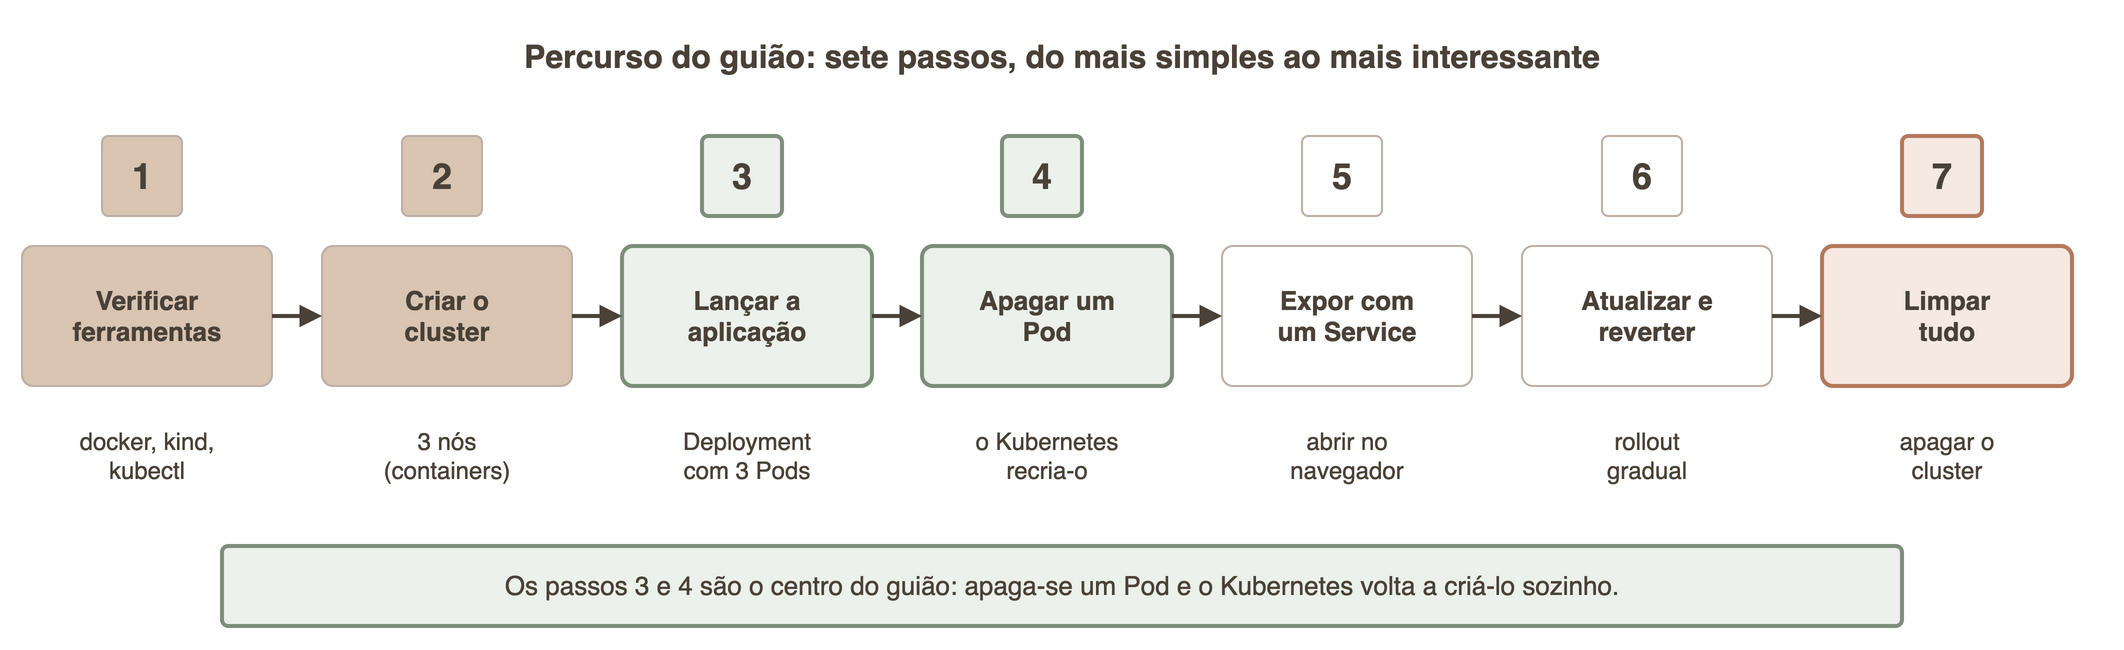
\includegraphics[width=\linewidth]{../Diagramas/g05-percurso.png}
\end{center}

\begin{leitura}
Os sete passos leem-se da esquerda para a direita. Os dois primeiros, a bege, preparam o ambiente: verificar as ferramentas e criar o cluster. Os passos 3 e 4, a verde, são a parte central: declara-se uma aplicação e observa-se a reação do Kubernetes quando um Pod é removido. Os passos 5 e 6, a branco, acrescentam o acesso à aplicação e a sua atualização. O passo 7, em tom avermelhado, encerra o trabalho e liberta os recursos. Abaixo de cada caixa, uma legenda resume o que é feito nesse passo.
\end{leitura}

\passo{1}{Verificação das ferramentas}

\textbf{Objetivo.} Confirmar que o Docker, o \cmd{kind} e o \cmd{kubectl} estão instalados e a funcionar.

\textbf{Enquadramento.} O \cmd{kind} cria o cluster utilizando containers Docker como nós. O \cmd{kubectl} é a ferramenta de linha de comandos através da qual se comunica com o cluster.

A figura mostra a relação entre as três ferramentas: o \cmd{kind} e o \cmd{kubectl} são programas instalados no computador, e o cluster que o \cmd{kind} cria existe dentro do Docker.

\begin{center}
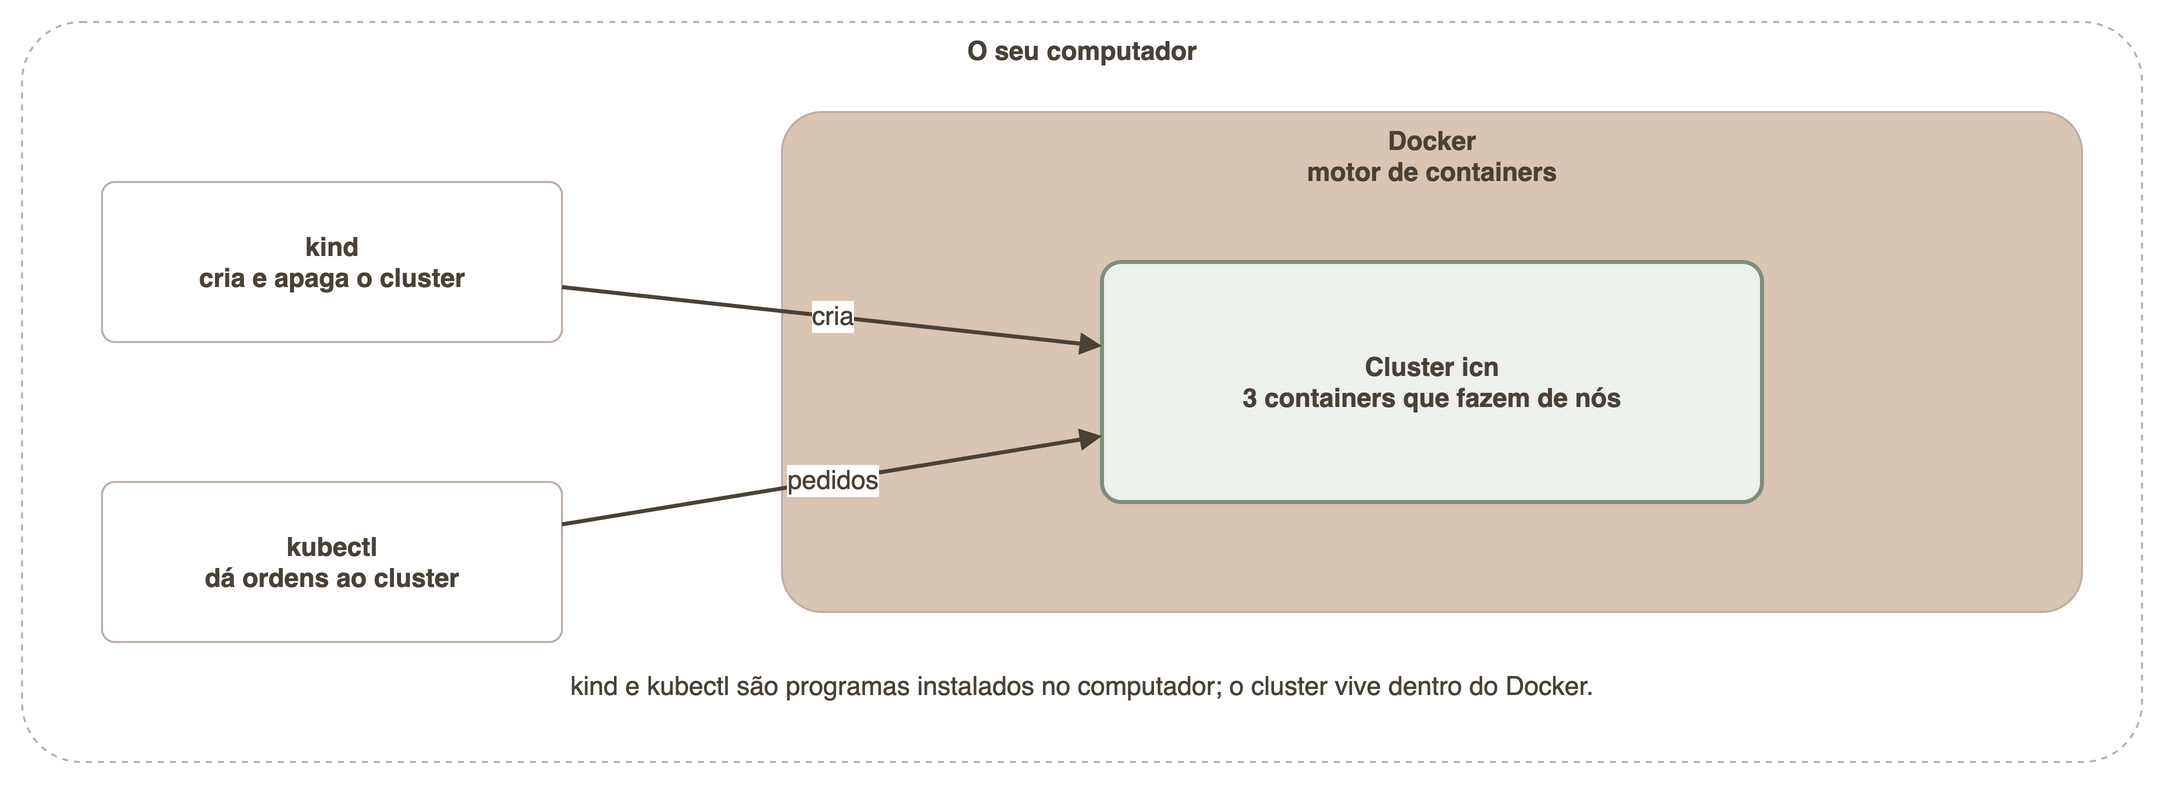
\includegraphics[width=\linewidth]{../Diagramas/g05-ferramentas.png}
\end{center}

\begin{leitura}
À esquerda estão os dois programas que o aluno utiliza: o \cmd{kind}, que cria e apaga o cluster, e o \cmd{kubectl}, que envia pedidos a um cluster já criado. À direita, a caixa maior representa o Docker e, dentro dela, a caixa verde representa o cluster, formado por três containers. A seta do \cmd{kind} indica que a criação é feita através do Docker. A seta do \cmd{kubectl} indica que os pedidos seguem diretamente para o cluster. Em resumo, as ferramentas ficam fora e o cluster vive dentro do Docker.
\end{leitura}

\begin{teoria}
O Kubernetes é, antes de mais, uma API. O \cmd{kubectl} é um cliente que traduz cada comando num pedido HTTP ao API server do cluster e apresenta a resposta. Para saber a que cluster falar e com que credenciais, lê o ficheiro kubeconfig, normalmente em \cmd{\textasciitilde/.kube/config}. Esse ficheiro guarda contextos. Cada contexto associa um cluster, um utilizador e, opcionalmente, um espaço de nomes. Ao criar um cluster, o \cmd{kind} acrescenta o contexto \cmd{kind-icn} e ativa-o. Por isso o comando \cmd{kubectl config use-context} resolve o erro de ligação recusada.

Os nós do \cmd{kind} não são uma versão reduzida do Kubernetes. São containers de sistema, no sentido da Aula 04: executam o \cmd{systemd} e, no seu interior, os mesmos componentes de um nó real, isto é, o kubelet, o \cmd{containerd} e, no nó de controlo, o API server, o etcd, o scheduler e o controller manager. Partilham o núcleo do anfitrião. Três nós custam, assim, muito menos memória do que três máquinas virtuais. Em Windows e macOS, esse núcleo é o da máquina virtual Linux do Docker Desktop.

\textbf{A analisar neste passo:} quem fala com quem. O \cmd{kind} e o \cmd{kubectl} são programas distintos, e só o segundo comunica com o cluster depois de este existir.
\end{teoria}

\subsection*{1.1 Abertura do terminal}

Em Windows, abrir o \textbf{PowerShell}. Em macOS, abrir o \textbf{Terminal}. Em Linux, abrir o terminal da distribuição.

\subsection*{1.2 Criação da pasta de trabalho}

Os dois ficheiros deste guião são guardados numa pasta própria.

\begin{terminal}
mkdir icn-aula05
cd icn-aula05
\end{terminal}

\subsection*{1.3 Verificação do Docker}

\begin{terminal}
docker --version
docker ps
\end{terminal}

\begin{saida}
Docker version 27.x.x, build abcdef1
CONTAINER ID   IMAGE   COMMAND   CREATED   STATUS   PORTS   NAMES
\end{saida}

A lista de containers pode estar vazia. O essencial é que os comandos não devolvam erro.

\begin{erro}
\textbf{Cannot connect to the Docker daemon} ou \textbf{error during connect}: o Docker não está em execução. Abrir o Docker Desktop e aguardar o estado \emph{running}. Em Linux, executar \cmd{sudo systemctl start docker}.

\textbf{permission denied while trying to connect} (Linux): o utilizador não pertence ao grupo \cmd{docker}. Executar \cmd{sudo usermod -aG docker \$USER}, terminar a sessão e iniciá-la de novo.

\textbf{docker: command not found}: o Docker não está instalado. Instalar o Docker Desktop (Windows e macOS) ou o Docker Engine (Linux), conforme \url{https://docs.docker.com/get-docker/}.
\end{erro}

\subsection*{1.4 Instalação do kind e do kubectl}

Deve ser seguida \textbf{apenas} a indicação correspondente ao sistema operativo em uso.

\textbf{macOS} (com Homebrew):

\begin{terminal}
brew install kind kubectl
\end{terminal}

\textbf{Windows} (PowerShell):

\begin{terminal}
winget install Kubernetes.kind
winget install Kubernetes.kubectl
\end{terminal}

No final, fechar o PowerShell e abrir outro, para que os comandos passem a ser reconhecidos.

\textbf{Linux}: seguir as instruções oficiais em \url{https://kind.sigs.k8s.io/docs/user/quick-start/} e em \url{https://kubernetes.io/docs/tasks/tools/}, que descrevem a obtenção de um único ficheiro executável.

\subsection*{1.5 Confirmação da instalação}

\begin{terminal}
kind version
kubectl version --client
\end{terminal}

\begin{saida}
kind v0.xx.x go1.xx.x darwin/arm64
Client Version: v1.xx.x
Kustomize Version: v5.x.x
\end{saida}

\begin{erro}
\textbf{kind: command not found} ou termo não reconhecido: fechar o terminal e abrir um novo. Se persistir, a pasta de instalação não consta da variável PATH; repetir a instalação e ler a mensagem final.

\textbf{brew: command not found}: instalar o Homebrew a partir de \url{https://brew.sh} ou usar a obtenção direta descrita nas páginas oficiais.
\end{erro}

\begin{feito}
Os comandos \cmd{docker ps}, \cmd{kind version} e \cmd{kubectl version -{}-client} executam sem erro.
\end{feito}

\passo{2}{Criação do cluster}

\textbf{Objetivo.} Descrever, num ficheiro, um cluster com três nós e solicitar ao \cmd{kind} a sua criação.

\textbf{Enquadramento.} Com um nó de controlo e dois nós de trabalho, é possível observar, mais adiante, a distribuição dos Pods por máquinas diferentes, tal como no diagrama da Aula 05.

\begin{center}
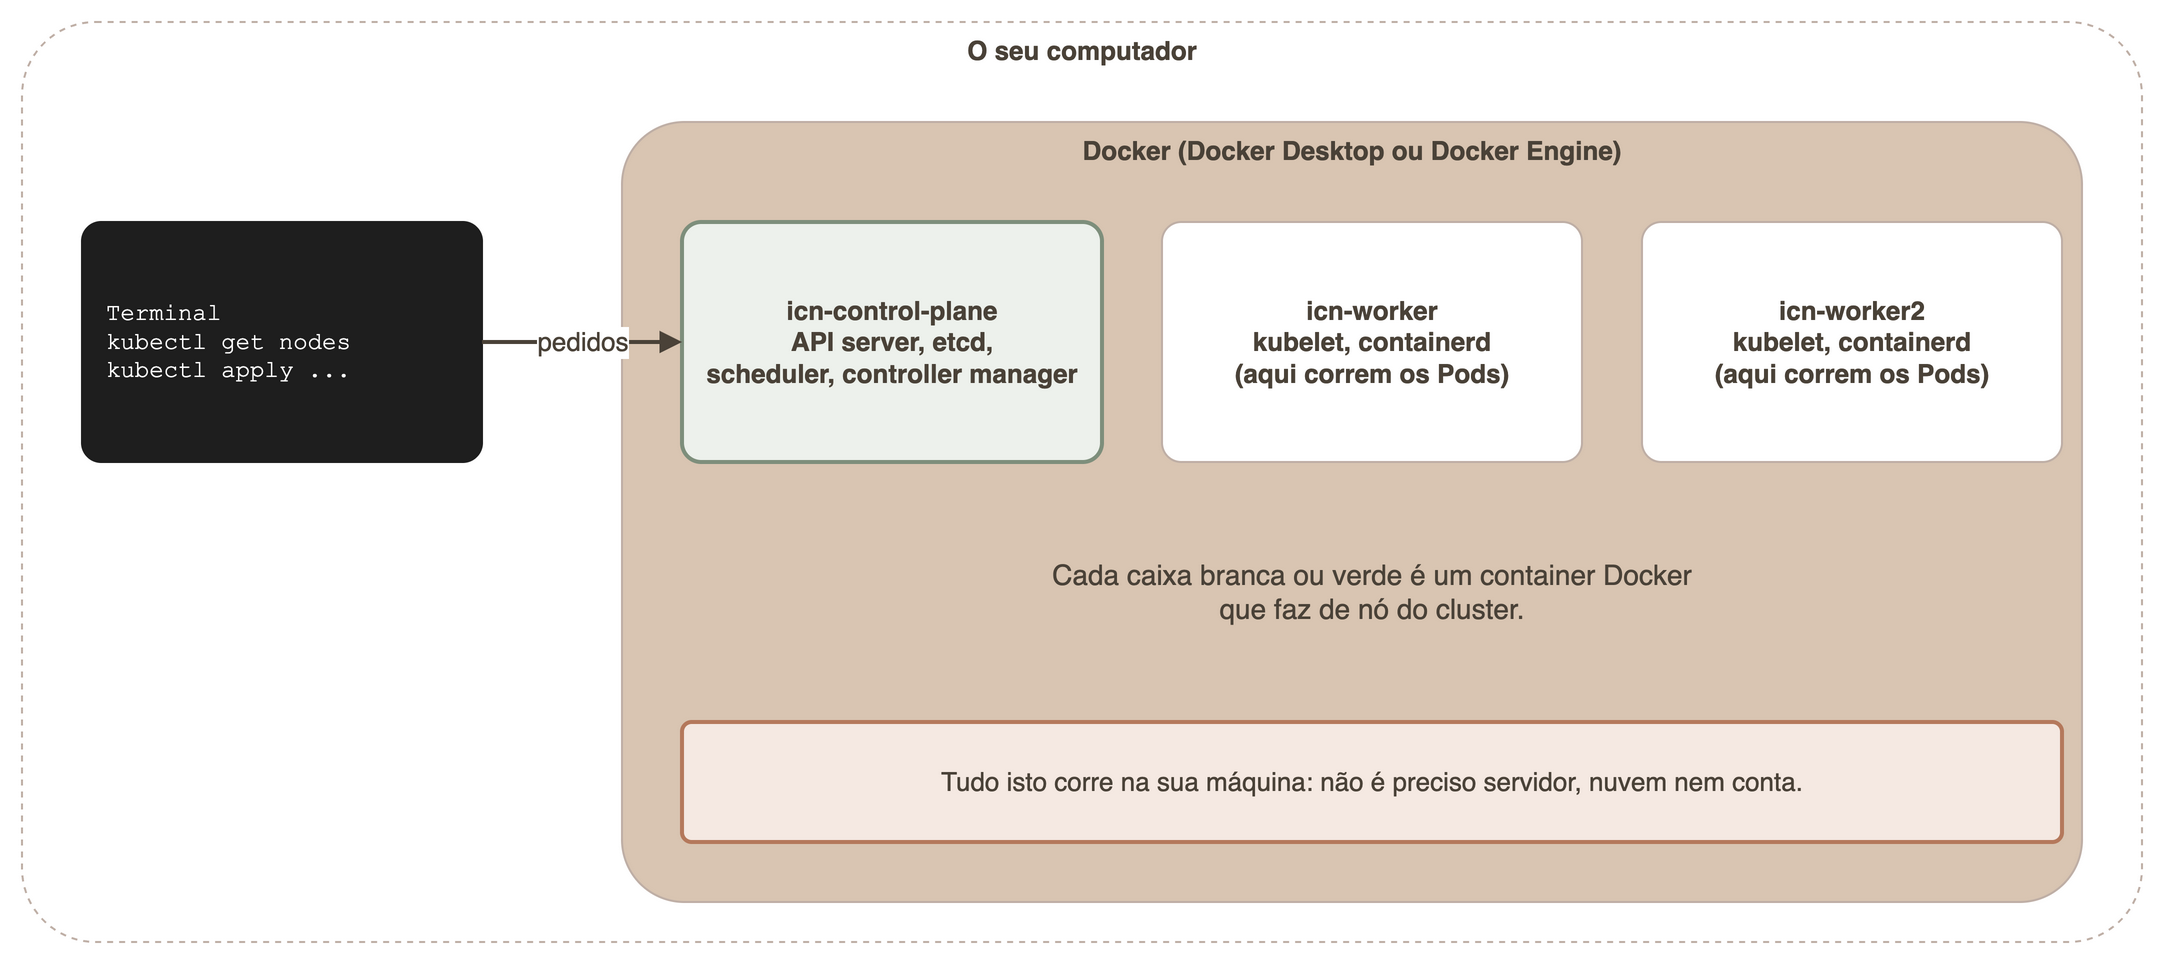
\includegraphics[width=\linewidth]{../Diagramas/g05-cluster.png}
\end{center}

\begin{leitura}
A figura detalha o que existe dentro do Docker no final deste passo. O nó de controlo, a verde, aloja os componentes que decidem: o API server, o etcd, o scheduler e o controller manager. Os dois nós de trabalho, a branco, executam os Pods, por intermédio do kubelet e do containerd. O terminal à esquerda representa o \cmd{kubectl}, cujos pedidos chegam sempre ao API server. Cada caixa corresponde a um dos três containers apresentados por \cmd{docker ps}.
\end{leitura}

\begin{teoria}
Um cluster divide-se em plano de controlo e nós de trabalho. No nó de controlo correm os componentes que decidem. Nos nós de trabalho correm as aplicações. Por omissão, o nó de controlo tem uma marca, um \emph{taint}, que impede o scheduler de lá colocar Pods comuns. É por isso que, neste laboratório, os Pods aparecem apenas nos dois nós de trabalho.

O estado \cmd{Ready} não significa apenas que a máquina está ligada. O kubelet comunica periodicamente com o API server e o nó só é declarado pronto quando o \emph{runtime} de containers funciona e a rede de Pods está configurada. Sem plugin de rede, o nó fica \cmd{NotReady}. O \cmd{kind} instala um plugin por omissão, e por isso o estado \cmd{Ready} surge sem passos adicionais.

A criação segue a sequência de um cluster real. O \cmd{kind} prepara os containers, inicia o nó de controlo com o \cmd{kubeadm} e junta depois os nós de trabalho. É a mesma ferramenta de arranque do diagrama de instalação apresentado na aula.

\textbf{A analisar neste passo:} a correspondência entre nós do Kubernetes e containers do Docker, e a diferença de papéis entre o nó de controlo e os restantes.
\end{teoria}

\subsection*{2.1 Ficheiro de configuração}

Criar, dentro da pasta \cmd{icn-aula05}, um ficheiro com o nome \cmd{kind-icn.yaml} e o conteúdo seguinte. Pode ser utilizado o Bloco de Notas (Windows: \cmd{notepad kind-icn.yaml}), o \cmd{nano} (macOS e Linux: \cmd{nano kind-icn.yaml}) ou outro editor de texto simples.

\begin{ficheiro}{kind-icn.yaml}
kind: Cluster
apiVersion: kind.x-k8s.io/v1alpha4
nodes:
  - role: control-plane
  - role: worker
  - role: worker
\end{ficheiro}

\begin{erro}
Os ficheiros YAML usam espaços, e não tabulações, para a indentação. Devem manter-se exatamente dois espaços antes de cada \cmd{- role}. Se o ficheiro for gravado como \cmd{kind-icn.yaml.txt}, o \cmd{kind} não o encontra: apagá-lo e gravar de novo com o nome correto.
\end{erro}

\subsection*{2.2 Criação do cluster}

A primeira execução demora entre dois e cinco minutos, por incluir a obtenção da imagem dos nós.

\begin{terminal}
kind create cluster --name icn --config kind-icn.yaml
\end{terminal}

\begin{saida}
Creating cluster "icn" ...
 Ensuring node image (kindest/node:v1.xx.x)
 Preparing nodes
 Writing configuration
 Starting control-plane
 Installing CNI
 Installing StorageClass
 Joining worker nodes
Set kubectl context to "kind-icn"
You can now use your cluster with:

kubectl cluster-info --context kind-icn
\end{saida}

Algumas linhas reais apresentam pequenos símbolos à esquerda, omitidos neste exemplo.

\begin{erro}
\textbf{node(s) already exist for a cluster with the name "icn"}: o cluster já foi criado anteriormente. Executar \cmd{kind delete cluster -{}-name icn} e repetir a criação.

\textbf{timed out waiting for the condition}, ou execução aparentemente parada: o Docker dispõe de pouca memória. Em Docker Desktop, abrir \emph{Settings}, depois \emph{Resources}, e atribuir pelo menos 4 GB. Aplicar, aguardar o reinício do Docker, apagar o cluster com o comando anterior e repetir.

\textbf{failed to pull image}, ou erros de rede: verificar a ligação à Internet e repetir. Em redes institucionais, pode ser necessário utilizar outra rede.
\end{erro}

\subsection*{2.3 Listagem dos nós}

\begin{terminal}
kubectl get nodes
\end{terminal}

\begin{saida}
NAME                  STATUS   ROLES           AGE   VERSION
icn-control-plane     Ready    control-plane   75s   v1.xx.x
icn-worker            Ready    <none>          55s   v1.xx.x
icn-worker2           Ready    <none>          55s   v1.xx.x
\end{saida}

Se algum nó apresentar o estado \textbf{NotReady}, aguardar cerca de meio minuto e repetir o comando.

\begin{erro}
\textbf{The connection to the server localhost:8080 was refused} ou \textbf{context not found}: o \cmd{kubectl} não está associado ao cluster. Executar \cmd{kubectl config use-context kind-icn} e repetir.
\end{erro}

\subsection*{2.4 Verificação de que os nós são containers}

\begin{terminal}
docker ps
\end{terminal}

\begin{saida}
CONTAINER ID   IMAGE                  STATUS         NAMES
3f1a9c2b7d10   kindest/node:v1.xx.x   Up 2 minutes   icn-worker2
8b7e6a5d4c31   kindest/node:v1.xx.x   Up 2 minutes   icn-worker
c0d9e8f7a6b5   kindest/node:v1.xx.x   Up 2 minutes   icn-control-plane
\end{saida}

\begin{observe}
O número de containers coincide com o número de nós listados no passo anterior. Cada nó do Kubernetes é, neste ambiente, um container Docker.

Recorde-se da Aula 04 que um container é um processo isolado por namespaces e limitado por cgroups. O cluster agora criado corre, portanto, sobre esse mesmo mecanismo.
\end{observe}

\begin{feito}
O comando \cmd{kubectl get nodes} apresenta três nós com o estado \textbf{Ready}.
\end{feito}

\passo{3}{Execução de uma aplicação}

\textbf{Objetivo.} Solicitar ao Kubernetes que mantenha três réplicas de um servidor web em execução.

\textbf{Enquadramento.} Trata-se do modo declarativo estudado na aula: não se indica como criar os Pods, mas qual o estado pretendido, cabendo ao Kubernetes atingi-lo e conservá-lo.

\begin{teoria}
Todo o objeto do Kubernetes tem a mesma estrutura de base. O campo \cmd{apiVersion} indica a versão da API, \cmd{kind} o tipo, \cmd{metadata} identifica o objeto e \cmd{spec} descreve o estado pretendido. Depois de criado, o objeto ganha um campo \cmd{status}, escrito pelo sistema, que regista o estado observado. A diferença entre \cmd{spec} e \cmd{status} é aquilo que os controladores procuram anular.

Um Deployment não cria Pods diretamente. Cria um ReplicaSet, cujo nome inclui um resumo do modelo de Pod, e é este que cria os Pods, com um sufixo aleatório. Daí a forma dos nomes, como \cmd{web-7c5ddbdd8d-4k8xq}: nome do Deployment, resumo do modelo, identificador do Pod. O \cmd{selector} e as etiquetas do modelo têm de coincidir, porque é assim que o ReplicaSet reconhece os Pods como seus.

O scheduler escolhe o nó de cada Pod em duas fases. Filtra os nós que não servem e pontua os restantes. Registada a escolha, o kubelet do nó obtém a imagem e inicia o container. A indicação \cmd{READY 1/1} significa que o único container do Pod está pronto.

O comando \cmd{kubectl apply} é idempotente. Aplicar o mesmo ficheiro duas vezes produz o mesmo resultado que aplicá-lo uma.

\textbf{A analisar neste passo:} a cadeia Deployment, ReplicaSet, Pod, e o facto de ter sido declarado um número e não uma sequência de ações.
\end{teoria}

\subsection*{3.1 Ficheiro da aplicação}

Criar, na mesma pasta, um ficheiro com o nome \cmd{web.yaml}.

\begin{ficheiro}{web.yaml}
apiVersion: apps/v1
kind: Deployment
metadata:
  name: web
spec:
  replicas: 3
  selector:
    matchLabels:
      app: web
  template:
    metadata:
      labels:
        app: web
    spec:
      containers:
        - name: nginx
          image: nginx:1.27
          ports:
            - containerPort: 80
\end{ficheiro}

O significado dos campos principais é o seguinte:

\begin{itemize}
  \item \cmd{kind: Deployment}: objeto que descreve uma aplicação gerida, aqui designada \cmd{web}.
  \item \cmd{replicas: 3}: número de cópias que devem existir em permanência.
  \item \cmd{app: web}: etiqueta atribuída a cada cópia, que permite ao Kubernetes reconhecê-las como pertencentes à aplicação.
  \item \cmd{image: nginx:1.27}: imagem do servidor web nginx, na versão 1.27, executada em cada cópia.
\end{itemize}

A figura associa cada linha relevante do ficheiro ao efeito que produz no cluster.

\begin{center}
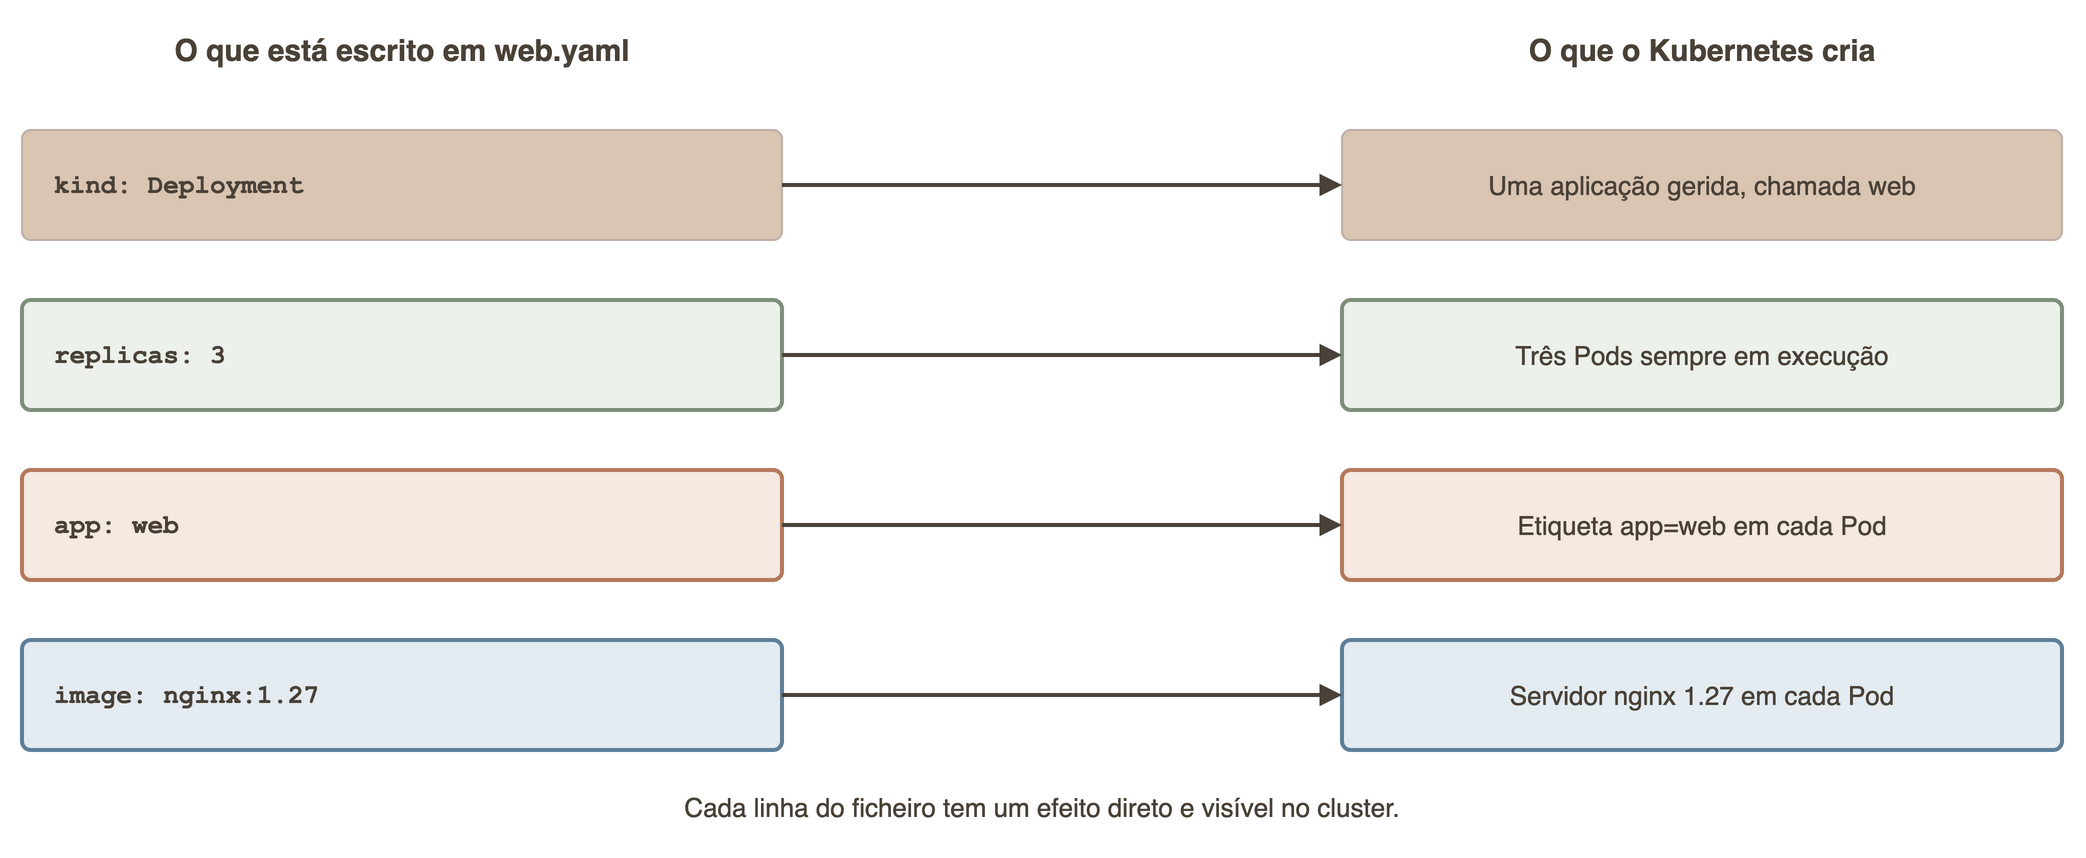
\includegraphics[width=\linewidth]{../Diagramas/g05-yaml.png}
\end{center}

\begin{leitura}
Cada linha do ficheiro, à esquerda, produz o efeito indicado à direita, com a mesma cor. A linha \cmd{kind: Deployment} determina o tipo de objeto. A linha \cmd{replicas: 3} define quantos Pods devem existir em permanência. A linha \cmd{app: web} é a etiqueta que cada Pod recebe, e é por ela que o ReplicaSet e, mais tarde, o Service reconhecem os Pods. A linha \cmd{image: nginx:1.27} indica a imagem executada em cada Pod. Alterar uma destas linhas e aplicar de novo o ficheiro altera o cluster em conformidade.
\end{leitura}

\subsection*{3.2 Aplicação do ficheiro}

\begin{terminal}
kubectl apply -f web.yaml
\end{terminal}

\begin{saida}
deployment.apps/web created
\end{saida}

\begin{erro}
\textbf{error converting YAML to JSON} ou \textbf{mapping values are not allowed}: existe um erro de indentação ou um carácter em excesso. Comparar o ficheiro com o do guião linha a linha e confirmar a utilização de espaços, e não de tabulações.

\textbf{error: the path "web.yaml" does not exist}: o terminal não se encontra na pasta do ficheiro. Executar \cmd{pwd} para verificar a localização e \cmd{cd icn-aula05} para entrar na pasta.
\end{erro}

\subsection*{3.3 Listagem dos Pods}

\begin{terminal}
kubectl get pods -o wide
\end{terminal}

\begin{saida}
NAME                   READY   STATUS    RESTARTS   AGE   IP           NODE
web-7c5ddbdd8d-4k8xq   1/1     Running   0          40s   10.244.1.2   icn-worker
web-7c5ddbdd8d-m2n7p   1/1     Running   0          40s   10.244.2.2   icn-worker2
web-7c5ddbdd8d-x9z4t   1/1     Running   0          40s   10.244.1.3   icn-worker
\end{saida}

Se o estado for \textbf{ContainerCreating}, a imagem ainda está a ser obtida. Aguardar alguns segundos e repetir.

\begin{erro}
\textbf{ImagePullBackOff} ou \textbf{ErrImagePull}: não foi possível obter a imagem. A causa surge na secção \emph{Events} do resultado de \cmd{kubectl describe pod <nome-do-pod>}. Corresponde, em regra, a falta de ligação à Internet ou a erro de escrita em \cmd{nginx:1.27}.

\textbf{Pending} durante muito tempo: normalmente, falta de memória ao Docker. Aumentá-la, conforme indicado no passo 2.
\end{erro}

\subsection*{3.4 Hierarquia de objetos}

\begin{terminal}
kubectl get deployment
kubectl get replicaset
\end{terminal}

\begin{saida}
NAME   READY   UP-TO-DATE   AVAILABLE   AGE
web    3/3     3            3           1m

NAME             DESIRED   CURRENT   READY   AGE
web-7c5ddbdd8d   3         3         3       1m
\end{saida}

\begin{observe}
Foi criado apenas um Deployment. Existe, contudo, um ReplicaSet com nome derivado do Deployment, e três Pods cujos nomes têm origem no nome desse ReplicaSet. Está assim visível a cadeia estudada na aula: Deployment, ReplicaSet, Pods.

Na coluna \textbf{NODE} do comando anterior, os Pods surgem repartidos pelos dois nós de trabalho. Essa decisão foi tomada pelo scheduler.
\end{observe}

\begin{feito}
Existem três Pods com o estado \textbf{Running} e a indicação \textbf{1/1}.
\end{feito}

\passo{4}{Remoção de um Pod}

\textbf{Objetivo.} Remover deliberadamente um dos Pods e observar a reação do Kubernetes.

\textbf{Enquadramento.} Este é o ponto central da aula. O Kubernetes compara continuamente o estado pretendido, três Pods, com o estado observado, e corrige qualquer diferença sem intervenção do utilizador.

\begin{center}
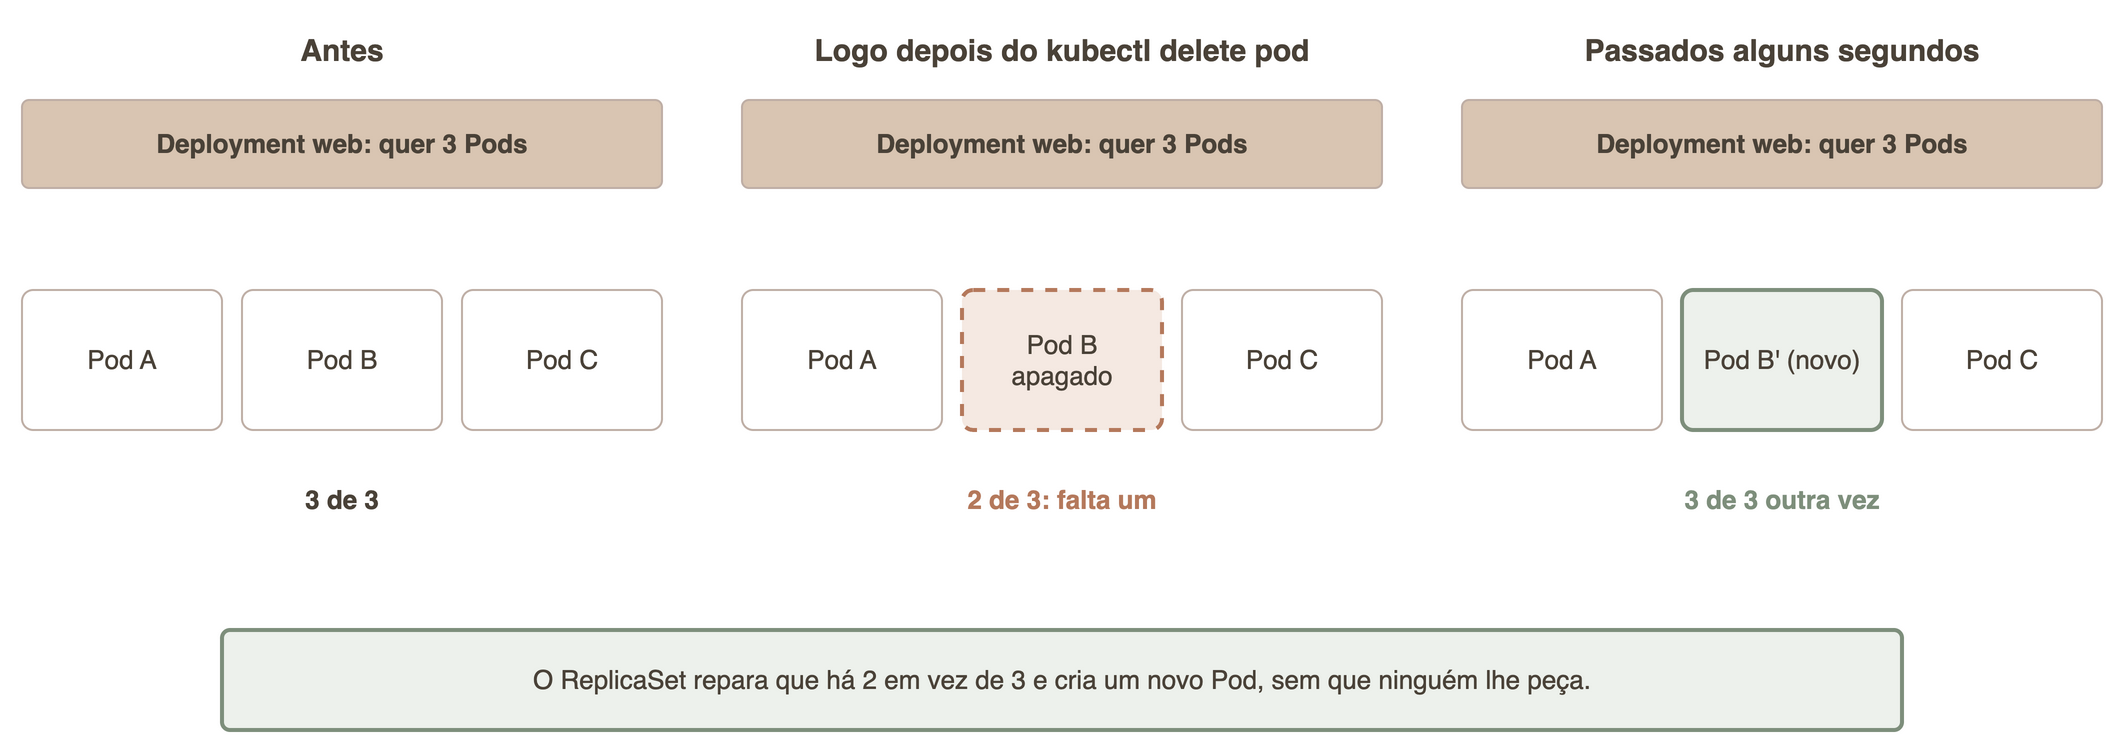
\includegraphics[width=\linewidth]{../Diagramas/g05-reconciliacao.png}
\end{center}

\begin{leitura}
A figura apresenta três instantes, da esquerda para a direita. No primeiro, o Deployment pretende três Pods e existem três. No segundo, imediatamente após o \cmd{kubectl delete pod}, o Pod B desapareceu e restam dois, o que contraria o estado pretendido. No terceiro, o ReplicaSet criou um Pod novo, designado B', e o número voltou a ser três. O Pod novo não é o antigo recuperado: tem outro nome e outro endereço IP.
\end{leitura}

\begin{teoria}
Um controlador é um ciclo que observa, compara e age. O do ReplicaSet observa os Pods que correspondem ao seu \emph{selector}, conta-os e compara a contagem com \cmd{replicas}. Se faltam, cria. Se sobram, elimina. Repete-o continuamente e reage ao estado, não ao evento: mesmo que perdesse a notificação da remoção, a contagem seguinte revelaria a diferença.

Remover um Pod é pedir ao API server que o marque para eliminação. O kubelet envia ao processo o sinal de terminação, aguarda por omissão até trinta segundos e, se o processo não terminar, força-o. É a fase \cmd{Terminating}. Entretanto, o ReplicaSet já criou o substituto, porque um Pod em eliminação deixou de contar.

O Pod novo é outro objeto, com outro nome e outro endereço IP. O Kubernetes não ressuscita Pods, substitui-os. Um Pod nunca deve, por isso, ser tratado como uma máquina com identidade própria.

Cada Pod guarda uma referência ao ReplicaSet que o criou. Se o ReplicaSet ou o Deployment fossem removidos, os Pods seriam eliminados em cascata. Remover só o Pod não altera o estado pretendido e, por isso, não tem efeito duradouro. A alteração do número de réplicas, como no ponto 4.4, atua sobre o estado pretendido e é tratada pelo mesmo ciclo.

\textbf{A analisar neste passo:} a sequência de estados no Terminal A, a diferença de nome e de IP antes e depois, e a razão pela qual o número final de Pods é o declarado.
\end{teoria}

Para acompanhar o processo, são utilizados \textbf{dois terminais} em simultâneo.

A figura representa a disposição: o Terminal A apenas observa, e o Terminal B emite a ordem de remoção.

\begin{center}
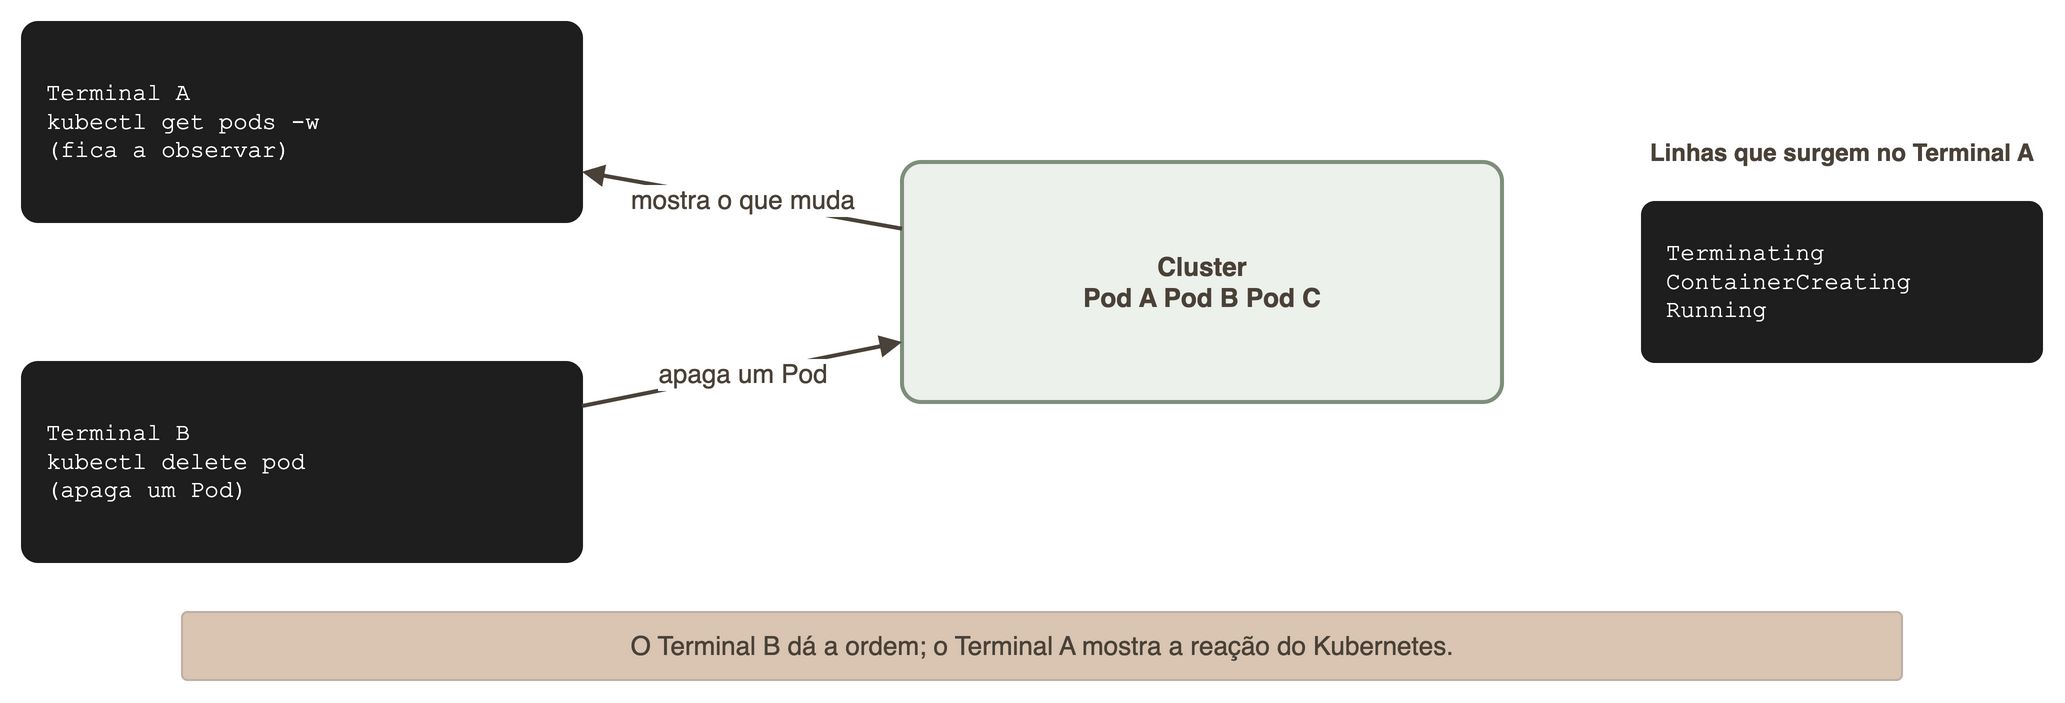
\includegraphics[width=\linewidth]{../Diagramas/g05-dois-terminais.png}
\end{center}

\begin{leitura}
A figura mostra a divisão de tarefas entre os dois terminais. O Terminal A executa \cmd{kubectl get pods -w} e limita-se a observar, sem alterar nada. O Terminal B emite a ordem de remoção. A seta de B para o cluster representa essa ordem, e a seta do cluster para A representa as linhas que o observador vai recebendo. A caixa da direita lista os estados que devem surgir no Terminal A, pela ordem habitual: \cmd{Terminating}, \cmd{ContainerCreating} e \cmd{Running}.
\end{leitura}

\subsection*{4.1 Terminal A: observação}

Abrir um novo terminal, entrar na pasta \cmd{icn-aula05} e executar:

\begin{terminal}
kubectl get pods -w
\end{terminal}

O comando permanece ativo e apresenta uma nova linha sempre que algo se altera. Deve ser mantido aberto.

\begin{saida}
NAME                   READY   STATUS    RESTARTS   AGE
web-7c5ddbdd8d-4k8xq   1/1     Running   0          6m
web-7c5ddbdd8d-m2n7p   1/1     Running   0          6m
web-7c5ddbdd8d-x9z4t   1/1     Running   0          6m
\end{saida}

\subsection*{4.2 Terminal B: remoção}

No outro terminal, escolher o nome de um Pod da lista e removê-lo, substituindo \cmd{<nome-do-pod>} pelo nome real, por exemplo \cmd{web-7c5ddbdd8d-4k8xq}.

\begin{terminal}
kubectl delete pod <nome-do-pod>
\end{terminal}

\begin{saida}
pod "web-7c5ddbdd8d-4k8xq" deleted
\end{saida}

\begin{nota}
Para copiar o nome do Pod, basta selecioná-lo com duplo clique no terminal. Muitos terminais completam também o nome com a tecla Tab, após a escrita das primeiras letras.
\end{nota}

\subsection*{4.3 Regresso ao Terminal A}

Em poucos segundos surgem novas linhas:

\begin{saida}
NAME                   READY   STATUS              RESTARTS   AGE
web-7c5ddbdd8d-4k8xq   1/1     Terminating         0          7m
web-7c5ddbdd8d-q7r2w   0/1     ContainerCreating   0          1s
web-7c5ddbdd8d-q7r2w   1/1     Running             0          3s
web-7c5ddbdd8d-4k8xq   0/1     Terminating         0          7m
\end{saida}

Concluída a observação, premir \textbf{Ctrl+C} no Terminal A para libertar o terminal.

\begin{observe}
Após a remoção de um Pod, voltam a existir três. O novo Pod não foi criado por solicitação do utilizador: foi o ReplicaSet que detetou a existência de dois Pods em vez de três e criou o que faltava.

O comando seguinte permite comparar o nome e o endereço IP do Pod novo com os do Pod removido.
\end{observe}

\begin{terminal}
kubectl get pods -o wide
\end{terminal}

Ambos diferem. O Kubernetes não repara um Pod, substitui-o por outro. Por esta razão, um Pod não deve ser referido pelo seu endereço, e é essa a questão que o Service do passo seguinte resolve.

\subsection*{4.4 Variação do número de réplicas}

O estado pretendido pode ser alterado com um único comando. Aumentar para cinco réplicas e observar o resultado:

\begin{terminal}
kubectl scale deployment web --replicas=5
kubectl get pods
\end{terminal}

Repor o valor original:

\begin{terminal}
kubectl scale deployment web --replicas=3
kubectl get pods
\end{terminal}

\begin{feito}
É possível explicar por que razão, após a remoção de um Pod, voltaram a existir três.
\end{feito}

\passo{5}{Exposição através de um Service}

\textbf{Objetivo.} Atribuir um ponto de acesso estável aos três Pods e aceder-lhe a partir do navegador.

\textbf{Enquadramento.} Os Pods são efémeros e mudam de endereço quando são substituídos. O Service constitui um ponto de entrada que se mantém.

\begin{center}
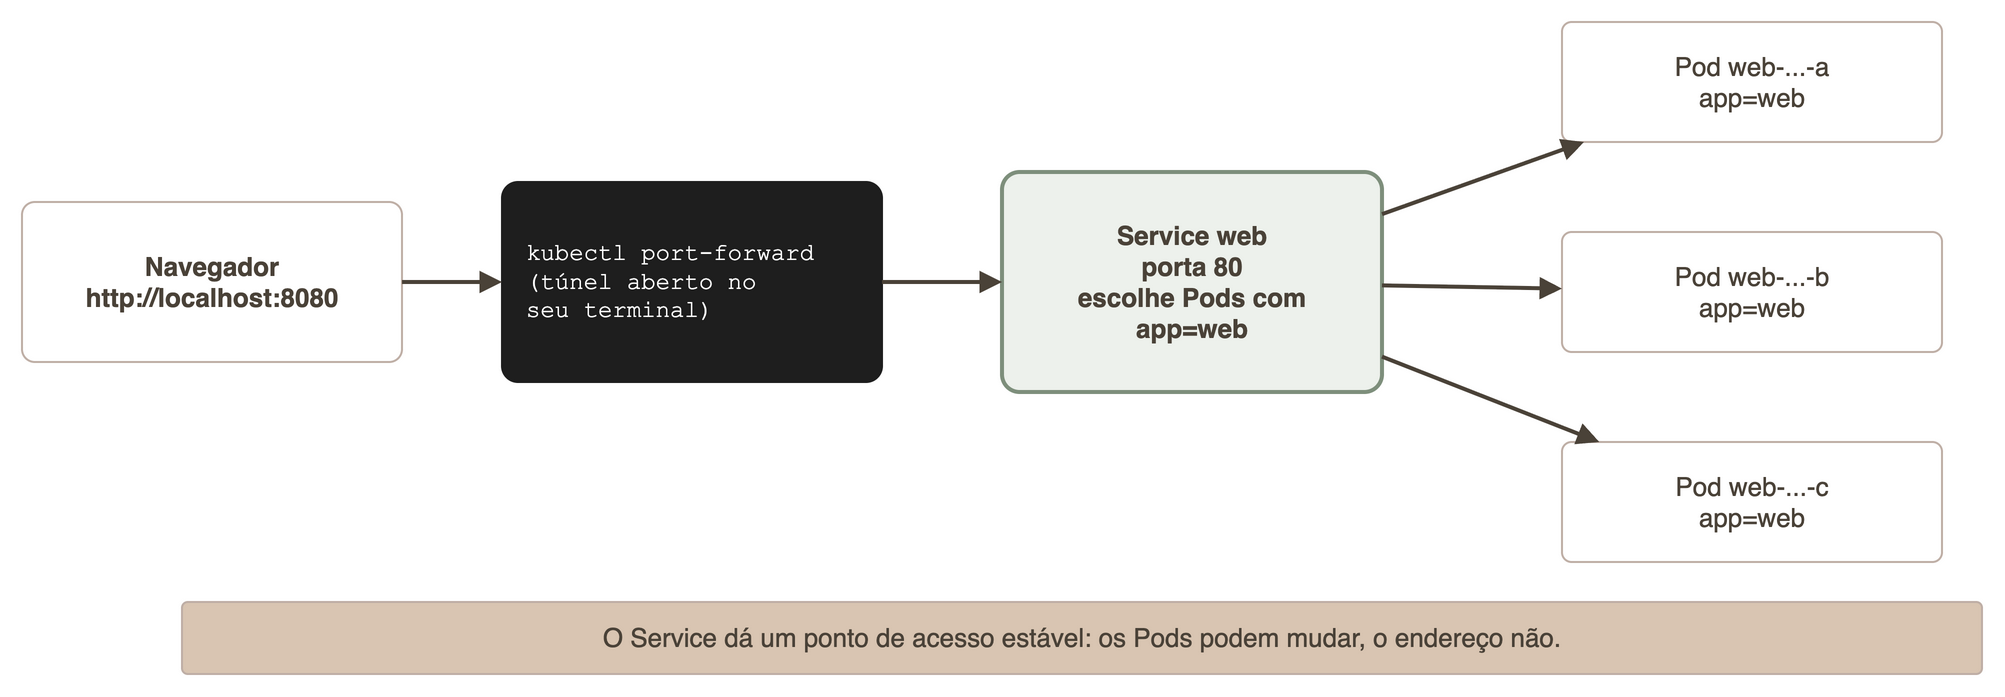
\includegraphics[width=\linewidth]{../Diagramas/g05-service.png}
\end{center}

\begin{leitura}
Lê-se da esquerda para a direita. O navegador acede ao endereço local \cmd{localhost:8080}. O comando \cmd{kubectl port-forward} mantém um túnel entre essa porta e um dos Pods do Service. O Service, que escuta na porta 80, seleciona os Pods com a etiqueta \cmd{app=web}, e o \cmd{kubectl} escolhe um deles quando abre o túnel. O túnel existe apenas para efeitos do laboratório, porque o Service é do tipo ClusterIP e só é acessível no interior do cluster. Os nomes dos Pods na figura são ilustrativos.
\end{leitura}

\begin{teoria}
Um Pod tem um endereço IP que muda quando o Pod é substituído. O Service resolve o problema com um endereço virtual estável, o ClusterIP, retirado de uma gama reservada ao cluster. Esse endereço não pertence a nenhuma interface. É implementado em cada nó pelo kube-proxy, que instala regras de rede a reescrever o destino para o endereço de um dos Pods.

A lista de destinos não é escrita à mão. Um controlador procura os Pods que satisfazem o \emph{selector} do Service e que estão prontos, e regista os seus endereços em objetos \emph{EndpointSlice}. Um Pod que falhe a sonda de \emph{readiness} sai da lista. Dentro do cluster, o Service pode ainda ser alcançado pelo nome, \cmd{web}, graças ao CoreDNS.

O tipo ClusterIP não é acessível do exterior. Existem o NodePort e o LoadBalancer para esse fim, mas aqui usa-se o \cmd{port-forward}, que é uma ferramenta de desenvolvimento. O \cmd{kubectl} liga-se ao API server, que reencaminha o tráfego até ao kubelet e daí ao Pod. Ao indicar um Service, o \cmd{kubectl} escolhe um dos Pods no momento em que abre o túnel, e todo o tráfego desse túnel segue para esse Pod. Atualizar a página não distribui, portanto, os pedidos pelos três.

\textbf{A analisar neste passo:} a correspondência entre os \emph{Endpoints} e os IP dos Pods, e o papel das etiquetas na ligação entre Service e Pods.
\end{teoria}

\subsection*{5.1 Criação do Service}

\begin{terminal}
kubectl expose deployment web --port=80
\end{terminal}

\begin{saida}
service/web exposed
\end{saida}

\begin{terminal}
kubectl get service web
\end{terminal}

\begin{saida}
NAME   TYPE        CLUSTER-IP     EXTERNAL-IP   PORT(S)   AGE
web    ClusterIP   10.96.123.45   <none>        80/TCP    10s
\end{saida}

O tipo é \textbf{ClusterIP}, pelo que o Service apenas é acessível no interior do cluster. Para lhe aceder a partir do navegador, é aberto um túnel temporário.

\subsection*{5.2 Abertura do túnel}

\begin{terminal}
kubectl port-forward service/web 8080:80
\end{terminal}

\begin{saida}
Forwarding from 127.0.0.1:8080 -> 80
Forwarding from [::1]:8080 -> 80
\end{saida}

O terminal fica ocupado enquanto o túnel estiver aberto, o que é o comportamento esperado. \textbf{Não deve ser fechado.}

\begin{erro}
\textbf{address already in use} ou \textbf{unable to listen on port 8080}: outra aplicação usa a porta 8080. Escolher outra, por exemplo \cmd{kubectl port-forward service/web 8081:80}, e aceder então a \cmd{http://localhost:8081}.

\textbf{unable to forward port because pod is not running}: os Pods ainda estão a arrancar. Aguardar e repetir.

\textbf{services "web" not found}: o Service não foi criado. Voltar ao ponto 5.1.
\end{erro}

\subsection*{5.3 Acesso pelo navegador}

Com o túnel aberto, introduzir no navegador o endereço:

\begin{terminal}
http://localhost:8080
\end{terminal}

Deve ser apresentada a página \textbf{Welcome to nginx!}. Concluído o acesso, premir \textbf{Ctrl+C} no terminal do túnel.

\begin{erro}
\textbf{A página não carrega}: confirmar que o terminal do túnel continua aberto e a apresentar \cmd{Forwarding from}. Caso tenha sido fechado, repetir o ponto 5.2.
\end{erro}

\subsection*{5.4 Destinos do tráfego}

\textbf{macOS e Linux:}

\begin{terminal}
kubectl describe service web | grep Endpoints
\end{terminal}

\textbf{Windows (PowerShell):}

\begin{terminal}
kubectl describe service web | Select-String Endpoints
\end{terminal}

\begin{saida}
Endpoints:  10.244.1.3:80,10.244.2.3:80,10.244.1.4:80
\end{saida}

A figura seguinte ilustra a seleção por etiquetas: o Service escolhe os Pods cuja etiqueta coincide com o seu \emph{selector} e ignora os restantes.

\begin{center}
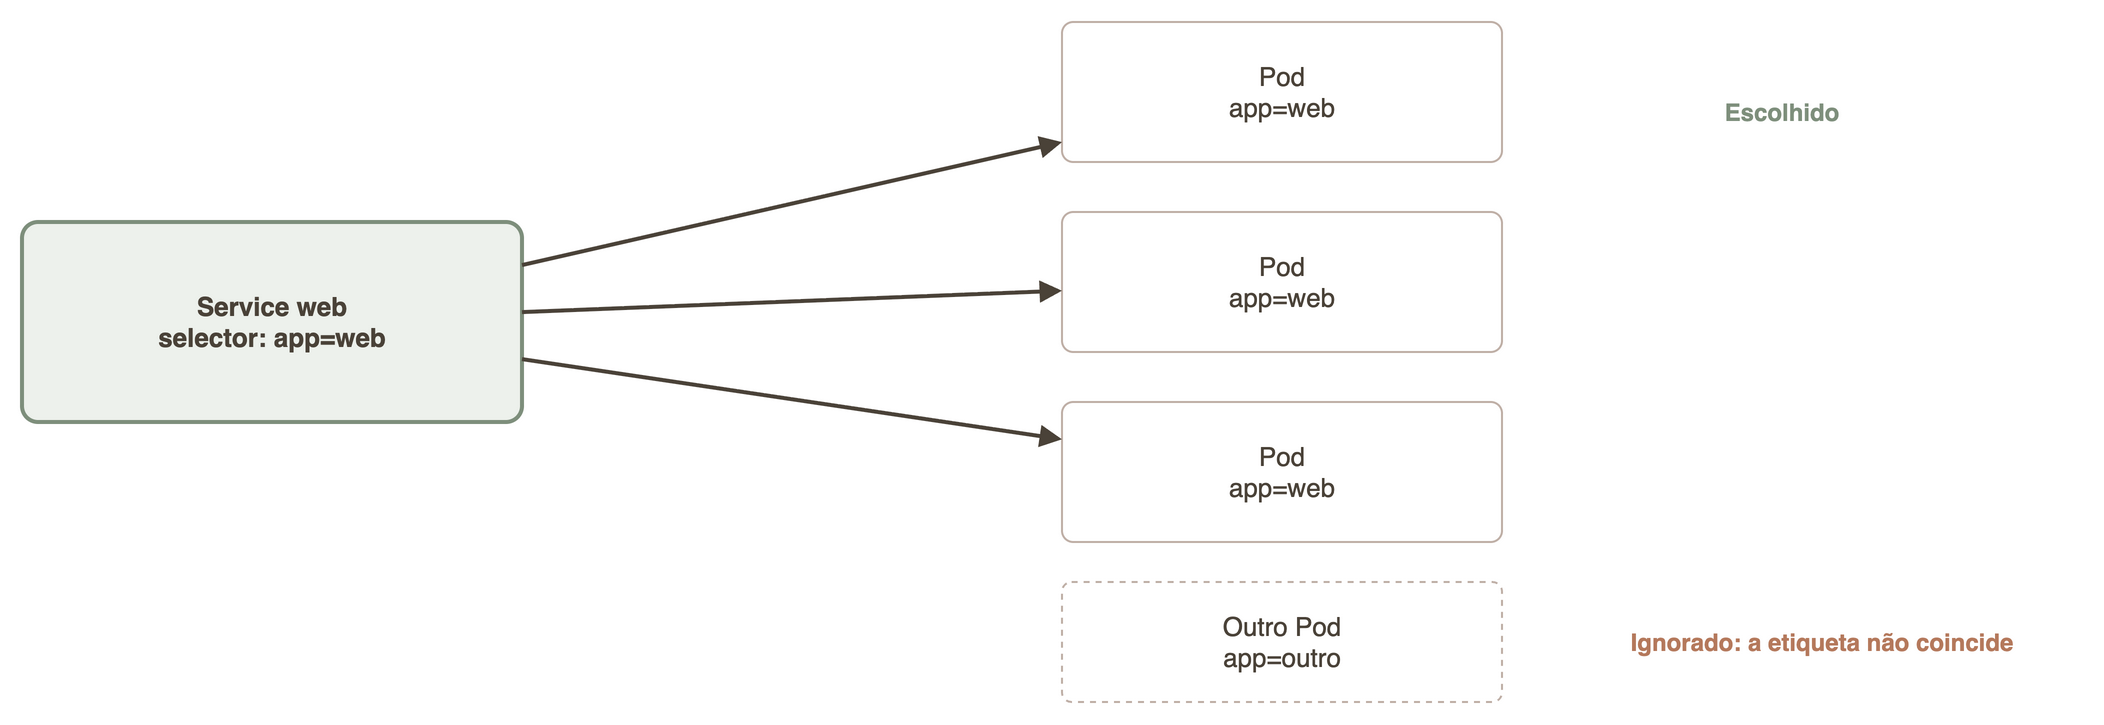
\includegraphics[width=\linewidth]{../Diagramas/g05-etiquetas.png}
\end{center}

\begin{leitura}
O Service não guarda uma lista de endereços. Guarda um critério, o \emph{selector} \cmd{app=web}, e seleciona em cada momento os Pods cuja etiqueta o satisfaz. Os três Pods com \cmd{app=web} são escolhidos. O Pod com \cmd{app=outro} é ignorado, mesmo estando no mesmo cluster. Se surgir um Pod novo com \cmd{app=web}, passa a ser escolhido, e se um desaparecer, deixa de o ser. É por esta razão que a lista de \emph{Endpoints} acompanha os Pods.
\end{leitura}

\begin{observe}
A lista contém três endereços, correspondentes aos da coluna \textbf{IP} do comando \cmd{kubectl get pods -o wide}, isto é, aos três Pods.

O Service não mantém uma lista escrita manualmente: seleciona os Pods pela etiqueta \cmd{app=web}. Quando um Pod desaparece, o seu endereço sai da lista e o do substituto entra.
\end{observe}

\begin{feito}
A página do nginx foi apresentada no navegador e é compreendida a origem da lista de \cmd{Endpoints}.
\end{feito}

\passo{6}{Atualização e reversão}

\textbf{Objetivo.} Substituir a versão do nginx de 1.27 para 1.28 sem interromper o serviço, e regressar à versão anterior.

\textbf{Enquadramento.} Cada versão de uma aplicação tem o seu ReplicaSet. O Kubernetes transita de um para o outro por etapas, mantendo sempre capacidade disponível.

\begin{center}
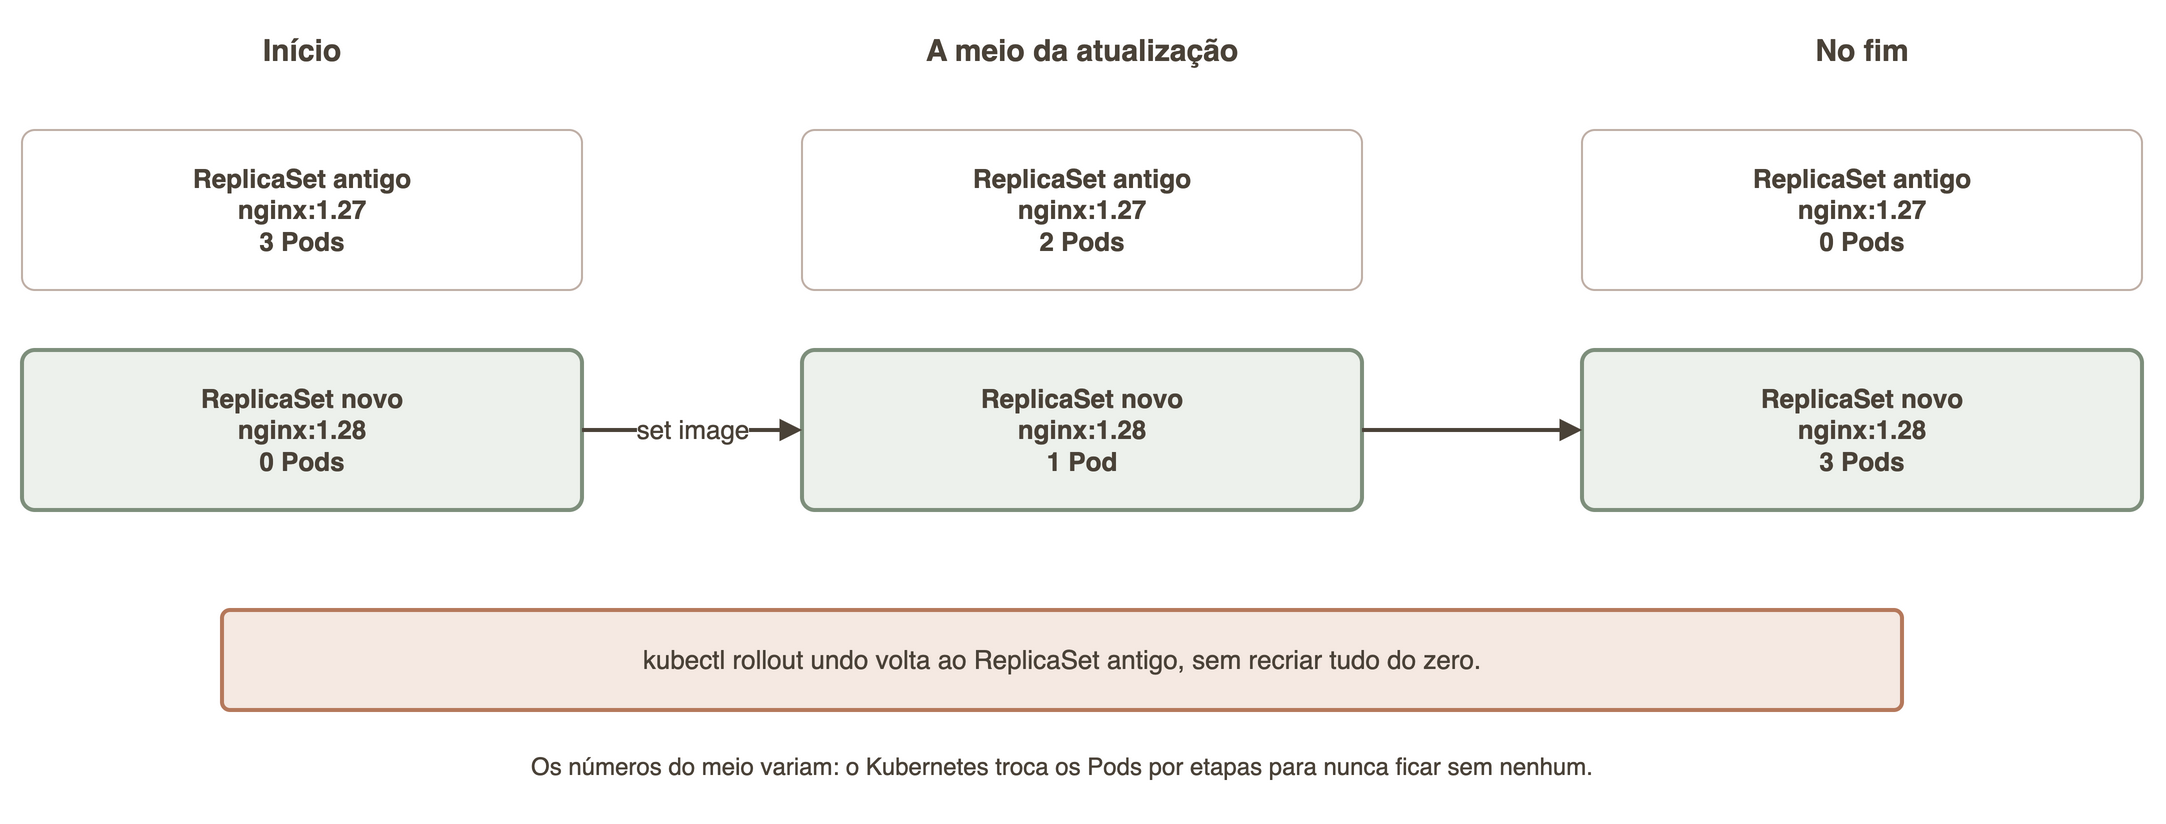
\includegraphics[width=\linewidth]{../Diagramas/g05-rollout.png}
\end{center}

\begin{leitura}
As três colunas representam três instantes da atualização. No início, o ReplicaSet antigo, com \cmd{nginx:1.27}, tem os três Pods e o novo, com \cmd{nginx:1.28}, não tem nenhum. A meio, o Kubernetes já criou um Pod da versão nova e retirou um da antiga, de modo que o serviço nunca fica sem Pods. No fim, todos os Pods são da versão nova e o ReplicaSet antigo ficou com zero. Este é conservado, e é por isso que o \cmd{kubectl rollout undo} é rápido. Os valores da coluna central são um exemplo e podem diferir.
\end{leitura}

\begin{teoria}
A atualização gradual é a estratégia por omissão do Deployment. O Kubernetes cria um ReplicaSet novo e transfere os Pods por etapas, reguladas por dois parâmetros: o número de Pods que podem existir acima do desejado, \cmd{maxSurge}, e o número que pode estar indisponível, \cmd{maxUnavailable}. Ambos valem por omissão vinte e cinco por cento, com arredondamento para cima no primeiro e para baixo no segundo. Com três réplicas, isto significa um Pod extra e nenhum indisponível. Cria-se um Pod novo, espera-se que fique pronto e só então se retira um antigo.

Sem sondas de \emph{readiness}, um Pod é considerado pronto assim que o container arranca. Em aplicações reais, a sonda impede que o tráfego chegue a um Pod ainda não preparado.

Os ReplicaSets antigos ficam, sem Pods, até um limite de dez revisões por omissão. A reversão não reconstrói nada: repõe no Deployment o modelo de Pod de uma revisão anterior.

Uma nota sobre o modo imperativo. O comando \cmd{kubectl set image} altera o objeto no cluster, mas não o ficheiro \cmd{web.yaml}, que continua a indicar a versão 1.27. Em contexto real, a alteração faz-se no ficheiro, que é a fonte de verdade, e aplica-se de novo.

\textbf{A analisar neste passo:} o número de Pods de cada ReplicaSet durante a atualização, e a diferença entre alterar o cluster por comando e alterar o ficheiro.
\end{teoria}

\subsection*{6.1 Atualização}

\begin{terminal}
kubectl set image deployment/web nginx=nginx:1.28
kubectl rollout status deployment/web
\end{terminal}

\begin{saida}
deployment.apps/web image updated
Waiting for deployment "web" rollout to finish: 1 out of 3 new replicas have been updated...
Waiting for deployment "web" rollout to finish: 2 out of 3 new replicas have been updated...
Waiting for deployment "web" rollout to finish: 1 old replicas are pending termination...
deployment "web" successfully rolled out
\end{saida}

\begin{erro}
\textbf{unable to find container named "nginx"}: o nome anterior ao sinal de igual deve ser o do container indicado em \cmd{web.yaml}, isto é, \cmd{nginx}.

\textbf{ImagePullBackOff} após a atualização: a versão solicitada não existe ou não foi possível obtê-la. Regressar à versão anterior com o comando do ponto 6.3.
\end{erro}

\subsection*{6.2 Os dois ReplicaSets}

\begin{terminal}
kubectl get replicaset
\end{terminal}

\begin{saida}
NAME             DESIRED   CURRENT   READY   AGE
web-7c5ddbdd8d   0         0         0       20m
web-6b8f9d4c5    3         3         3       1m
\end{saida}

\begin{observe}
Existem agora dois ReplicaSets: o antigo ficou sem Pods e o novo mantém três.

O ReplicaSet antigo não foi removido. Conserva a descrição da versão anterior, razão pela qual o regresso a essa versão é rápido.
\end{observe}

\subsection*{6.3 Reversão}

\begin{terminal}
kubectl rollout undo deployment/web
kubectl rollout status deployment/web
\end{terminal}

\begin{saida}
deployment.apps/web rolled back
deployment "web" successfully rolled out
\end{saida}

Confirmar a imagem em uso:

\textbf{macOS e Linux:}

\begin{terminal}
kubectl describe deployment web | grep Image
\end{terminal}

\textbf{Windows (PowerShell):}

\begin{terminal}
kubectl describe deployment web | Select-String Image
\end{terminal}

\begin{saida}
    Image:        nginx:1.27
\end{saida}

\begin{feito}
A aplicação passou de \cmd{nginx:1.27} para \cmd{nginx:1.28} e regressou a \cmd{nginx:1.27}, sem remoção manual de qualquer objeto.
\end{feito}

\section*{Desafio opcional: perda de um nó}

Este desafio é facultativo, deve ser realizado apenas se o tempo o permitir e enquanto o cluster existir. Demora cerca de dez minutos.

A figura apresenta a sequência temporal esperada, desde a paragem do nó até à criação de Pods substitutos.

\begin{center}
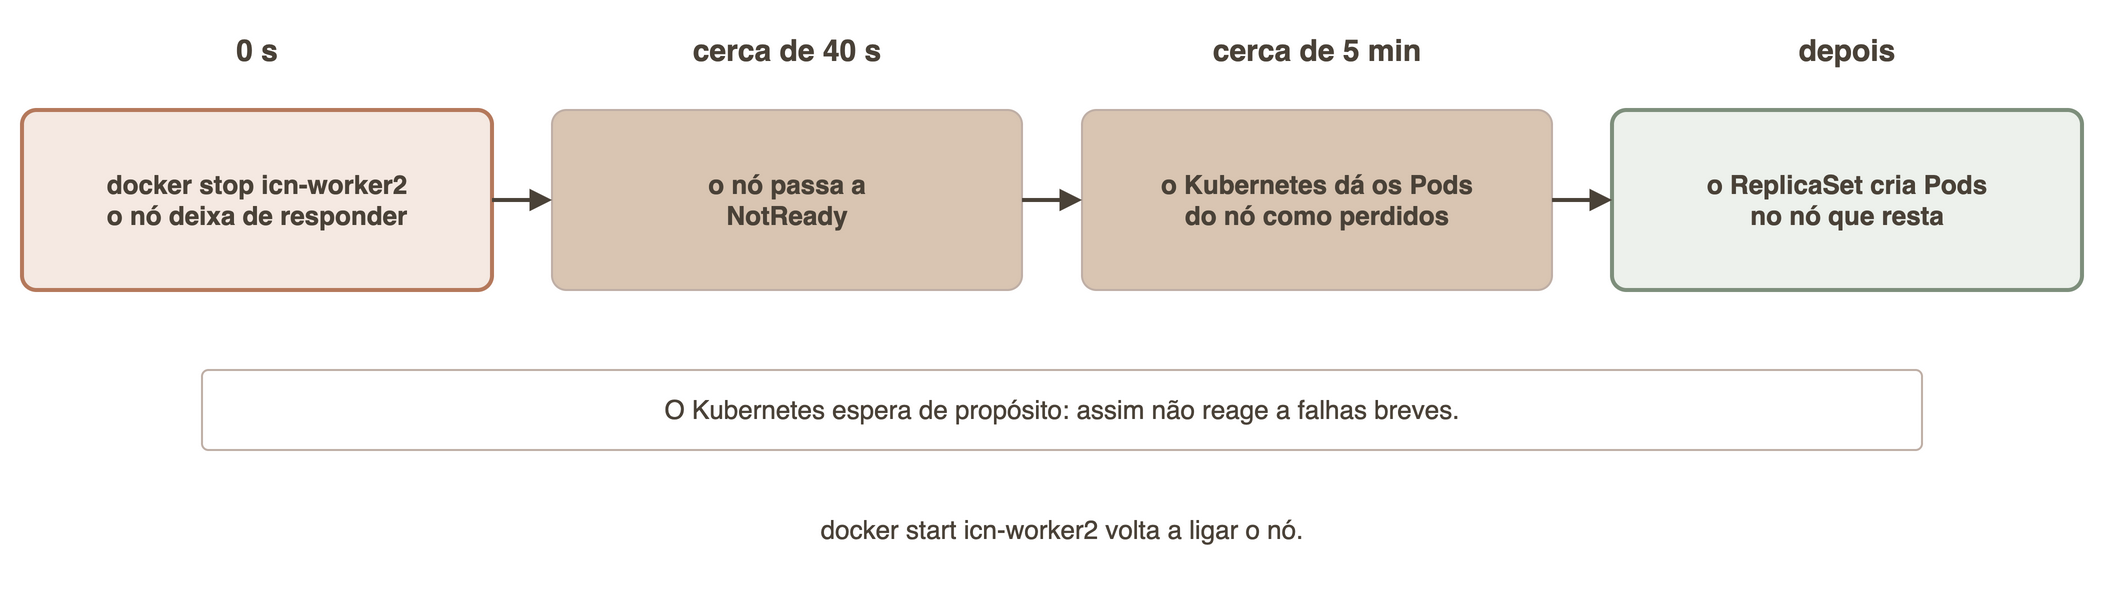
\includegraphics[width=\linewidth]{../Diagramas/g05-no-perdido.png}
\end{center}

\begin{leitura}
A sequência lê-se da esquerda para a direita. Ao parar o container do nó, este deixa de comunicar com o plano de controlo. Cerca de quarenta segundos depois, o nó é marcado como \cmd{NotReady}. Os Pods que nele estavam não são substituídos de imediato, porque o Kubernetes tolera, por omissão, cerca de cinco minutos de ausência antes de os dar como perdidos. Só então o ReplicaSet cria substitutos no nó que continua disponível. Os tempos são valores por omissão e podem variar.
\end{leitura}

\begin{teoria}
O kubelet de cada nó renova periodicamente, por omissão a cada dez segundos, um registo de presença no API server. Quando esses registos deixam de chegar durante cerca de quarenta segundos, o controlador de nós marca o nó como inacessível e o estado passa a \cmd{NotReady}. O controlador acrescenta então ao nó uma marca do tipo \cmd{NoExecute}, que repele Pods.

Os Pods recebem automaticamente uma tolerância a essa marca durante trezentos segundos. Só depois são expulsos, e só então o ReplicaSet cria substitutos noutro nó. Entretanto, o kubelet do nó parado não pode terminar os Pods, e o estado que o cluster conhece deles é o último que foi comunicado.

A espera é uma decisão de desenho. Reagir de imediato encurtaria a interrupção, mas faria o cluster tratar uma falha de rede de poucos segundos como uma avaria e deslocar cargas sem necessidade. Há também uma razão de correção. Sem saber se o nó está de facto parado, o Kubernetes arriscaria ter duas instâncias do mesmo Pod ativas ao mesmo tempo, o que é perigoso em aplicações com estado. Quem precisa de reagir mais depressa pode ajustar a tolerância por Pod.

\textbf{A analisar neste desafio:} os tempos observados e a relação entre disponibilidade e prudência.
\end{teoria}

\textbf{1.} Verificar em que nós se encontram os Pods.

\begin{terminal}
kubectl get pods -o wide
\end{terminal}

\textbf{2.} Parar um dos nós de trabalho, simulando a avaria da máquina.

\begin{terminal}
docker stop icn-worker2
\end{terminal}

\textbf{3.} Observar o estado dos nós.

\begin{terminal}
kubectl get nodes -w
\end{terminal}

Passado cerca de meio minuto, o estado do nó passa a \textbf{NotReady}.

\begin{saida}
NAME                  STATUS     ROLES           AGE   VERSION
icn-control-plane     Ready      control-plane   30m   v1.xx.x
icn-worker            Ready      <none>          30m   v1.xx.x
icn-worker2           NotReady   <none>          30m   v1.xx.x
\end{saida}

\begin{observe}
Os Pods do nó parado não são recriados de imediato. Por omissão, o Kubernetes aguarda cerca de cinco minutos antes de os considerar perdidos, de modo a não reagir a falhas breves. Decorrido esse tempo, o ReplicaSet cria substitutos no nó que se mantém disponível.

Premir Ctrl+C para sair do modo de observação e repetir \cmd{kubectl get pods -o wide} periodicamente.
\end{observe}

\textbf{4.} Concluída a observação, voltar a iniciar o nó.

\begin{terminal}
docker start icn-worker2
\end{terminal}

\passo{7}{Remoção do cluster}

\textbf{Objetivo.} Eliminar o cluster, libertando a memória e o espaço em disco utilizados.

A figura mostra o que é removido e o que permanece após a eliminação do cluster.

\begin{center}
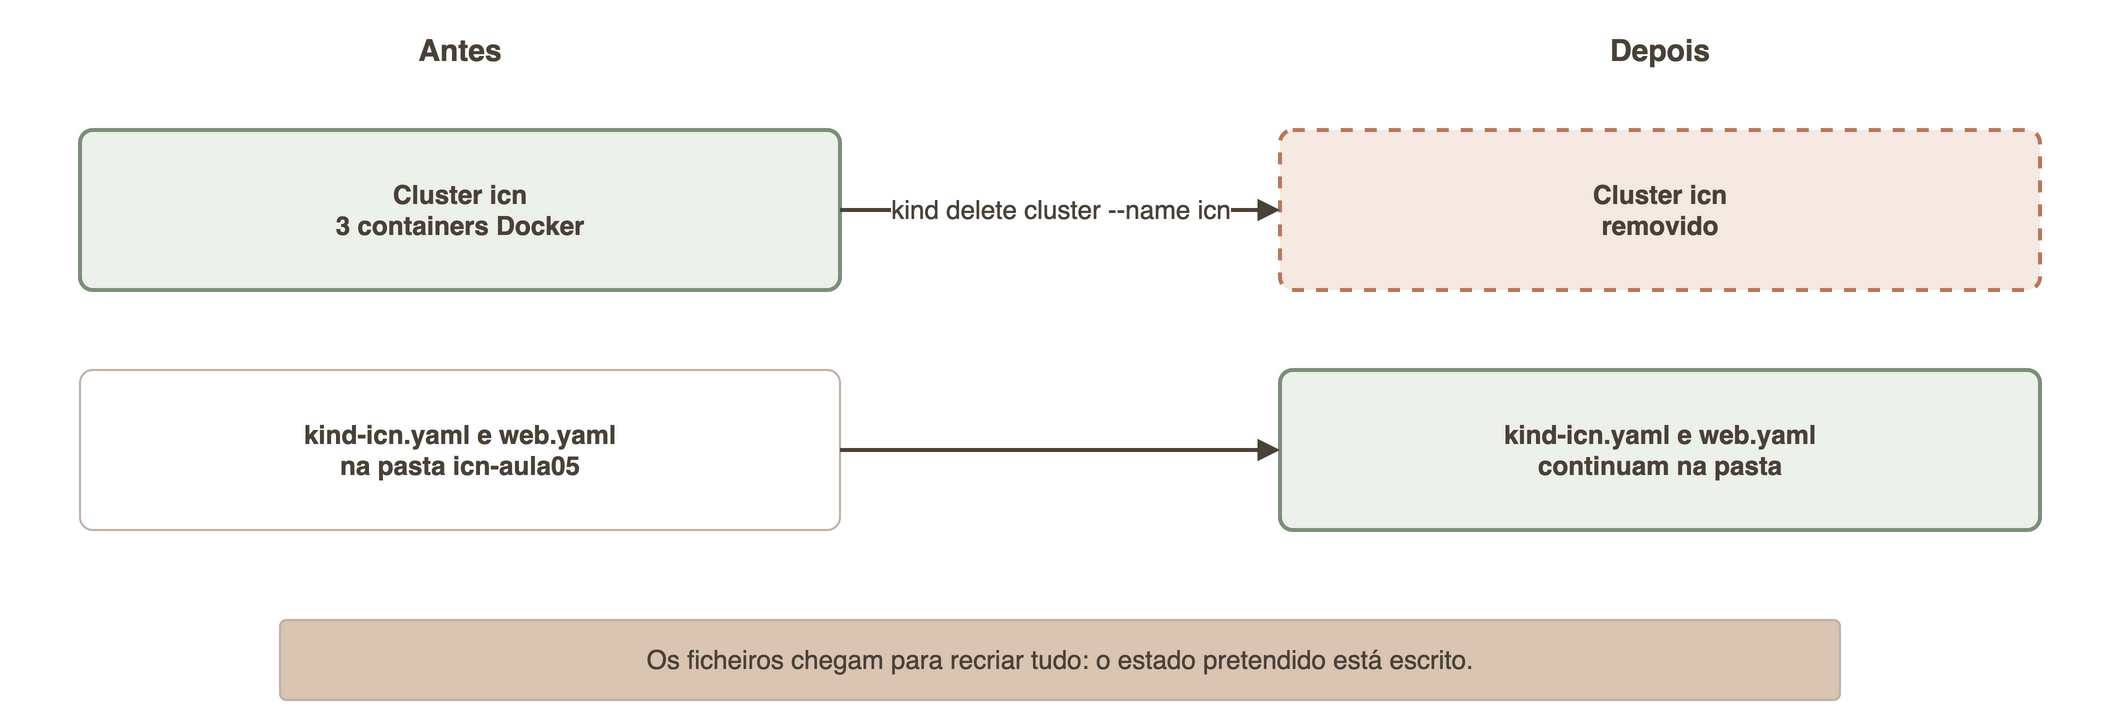
\includegraphics[width=\linewidth]{../Diagramas/g05-limpeza.png}
\end{center}

\begin{leitura}
A figura compara o ambiente antes e depois do comando \cmd{kind delete cluster}. O cluster, composto por três containers Docker, é removido por completo, incluindo os Pods, os Deployments e os Services nele criados. Os dois ficheiros YAML, que estão numa pasta do computador e não dentro do cluster, permanecem. Com eles é possível recriar o mesmo ambiente com dois comandos, o que ilustra a vantagem de descrever o estado pretendido em ficheiros.
\end{leitura}

\begin{teoria}
O estado do cluster vive no etcd, que neste laboratório está dentro do container do nó de controlo. Eliminar o cluster elimina esses containers e, com eles, todos os objetos criados: Deployments, ReplicaSets, Pods e Services. Não há nada a desfazer objeto a objeto.

Sobrevive o que está fora do cluster. Os ficheiros \cmd{kind-icn.yaml} e \cmd{web.yaml} descrevem o cluster e a aplicação e bastam para os recriar. Esta é a ideia da infraestrutura descrita como código, que a Aula 07 aprofunda. O estado pretendido fica escrito, versionável e reproduzível, e o ambiente concreto passa a ser descartável.

A imagem dos nós fica na cache do Docker, o que acelera a criação seguinte. Pode ser removida com \cmd{docker image rm} se for preciso libertar espaço.

\textbf{A analisar neste passo:} o que deixou de existir e o que continua a permitir recriá-lo.
\end{teoria}

\subsection*{7.1 Eliminação}

\begin{terminal}
kind delete cluster --name icn
\end{terminal}

\begin{saida}
Deleting cluster "icn" ...
Deleted nodes: ["icn-worker2" "icn-worker" "icn-control-plane"]
\end{saida}

\subsection*{7.2 Verificação}

\begin{terminal}
docker ps
\end{terminal}

\begin{saida}
CONTAINER ID   IMAGE   COMMAND   CREATED   STATUS   PORTS   NAMES
\end{saida}

Não deve surgir nenhum container \cmd{kindest/node}. Os ficheiros \cmd{kind-icn.yaml} e \cmd{web.yaml} permanecem na pasta e permitem reconstruir o ambiente em poucos minutos.

\begin{nota}
Para repetir o laboratório, bastam os comandos \cmd{kind create cluster -{}-name icn -{}-config kind-icn.yaml} e \cmd{kubectl apply -f web.yaml}. É esta a vantagem do modo declarativo: o estado pretendido fica escrito e é reproduzível.
\end{nota}

\clearpage
\section*{Resolução de problemas: consulta rápida}

\renewcommand{\arraystretch}{1.7}
\begin{center}
\small
\begin{tabular}{>{\raggedright\arraybackslash}p{5.6cm} >{\raggedright\arraybackslash}p{9.2cm}}
\toprule
\textbf{Sintoma} & \textbf{Resolução} \\
\midrule
\cmd{Cannot connect to the Docker daemon} & Abrir o Docker Desktop e aguardar o estado \emph{running}. Em Linux, \cmd{sudo systemctl start docker}. \\
\cmd{permission denied} (Docker, Linux) & \cmd{sudo usermod -aG docker \$USER}, terminar a sessão e iniciá-la de novo. \\
\cmd{command not found} ou termo não reconhecido & Fechar e abrir o terminal. Se persistir, repetir a instalação da ferramenta. \\
\cmd{node(s) already exist ... "icn"} & \cmd{kind delete cluster -{}-name icn} e repetir a criação. \\
Criação do cluster parada ou \cmd{timed out} & Atribuir pelo menos 4 GB de memória ao Docker, apagar o cluster e repetir. \\
\cmd{connection to the server ... refused} & \cmd{kubectl config use-context kind-icn} \\
Nó em \cmd{NotReady} & Aguardar meio minuto e repetir \cmd{kubectl get nodes}. \\
\cmd{error converting YAML to JSON} & Rever a indentação: apenas espaços, sem tabulações, igual ao guião. \\
\cmd{the path "web.yaml" does not exist} & Confirmar a pasta com \cmd{pwd} e entrar com \cmd{cd icn-aula05}. \\
\cmd{ContainerCreating} durante muito tempo & A imagem ainda está a ser obtida. Aguardar e repetir. \\
\cmd{ImagePullBackOff} ou \cmd{ErrImagePull} & \cmd{kubectl describe pod <nome>} e ler \emph{Events}. Verificar a Internet e o nome da imagem. \\
Pod em \cmd{Pending} & Recursos insuficientes. Aumentar a memória do Docker. \\
\cmd{address already in use} & Usar outra porta local, por exemplo \cmd{8081:80}. \\
A página não abre no navegador & O terminal do \cmd{port-forward} tem de permanecer aberto. \\
Cluster ativo desconhecido & \cmd{kubectl config get-contexts} \\
\bottomrule
\end{tabular}
\end{center}

\section*{Comandos utilizados}

\begin{center}
\small
\begin{tabular}{>{\raggedright\arraybackslash}p{7.2cm} >{\raggedright\arraybackslash}p{7.6cm}}
\toprule
\textbf{Comando} & \textbf{Finalidade} \\
\midrule
\cmd{kind create cluster -{}-name icn -{}-config kind-icn.yaml} & Criar o cluster de três nós \\
\cmd{kubectl get nodes} & Listar os nós \\
\cmd{kubectl apply -f web.yaml} & Aplicar o estado pretendido descrito no ficheiro \\
\cmd{kubectl get pods -o wide} & Listar Pods, com endereço IP e nó \\
\cmd{kubectl get pods -w} & Observar alterações em tempo real \\
\cmd{kubectl delete pod <nome>} & Remover um Pod \\
\cmd{kubectl scale deployment web -{}-replicas=5} & Alterar o número de réplicas \\
\cmd{kubectl expose deployment web -{}-port=80} & Criar um Service \\
\cmd{kubectl port-forward service/web 8080:80} & Abrir um túnel para o navegador \\
\cmd{kubectl describe <tipo> <nome>} & Apresentar o detalhe e os eventos de um objeto \\
\cmd{kubectl set image deployment/web nginx=nginx:1.28} & Atualizar a imagem \\
\cmd{kubectl rollout status deployment/web} & Acompanhar uma atualização \\
\cmd{kubectl rollout undo deployment/web} & Regressar à versão anterior \\
\cmd{kind delete cluster -{}-name icn} & Eliminar o cluster \\
\bottomrule
\end{tabular}
\end{center}

\section*{Síntese}

O laboratório permitiu observar, na prática, as ideias centrais da Aula 05:

\begin{itemize}
  \item Um \textbf{cluster} é um conjunto de nós; neste ambiente, cada nó era um container Docker.
  \item O \textbf{Deployment} declara o estado pretendido e o \textbf{ReplicaSet} mantém o número de Pods.
  \item A remoção de um Pod não o elimina de forma duradoura, porque o Kubernetes \textbf{reconcilia} o estado pretendido com o observado.
  \item Os Pods são efémeros, e o \textbf{Service} oferece-lhes um ponto de acesso estável, selecionando-os por \textbf{etiquetas}.
  \item A \textbf{atualização gradual} transita entre ReplicaSets por etapas, e o \textbf{rollout undo} repõe a versão anterior.
\end{itemize}

\end{document}
